\documentclass[11pt,letterpaper]{article}
% Preamble for "Critical mean out-degrees of lattice neighbour graphs"
\IfFileExists{lmodern.sty}{\usepackage[T1]{fontenc}\usepackage{lmodern}}{}
\usepackage[british]{babel}
\usepackage{amsmath,amsthm,amssymb,mathtools}
\usepackage[margin=1.05in]{geometry}
\usepackage{microtype}
\setlength{\emergencystretch}{1em}
\usepackage{xcolor}
\definecolor{paperlink}{RGB}{0,0,114}
\usepackage{tikz}
\usetikzlibrary{arrows.meta,decorations.pathmorphing}
\usepackage{booktabs}
\usepackage{hyperref}
\hypersetup{colorlinks=true,linktoc=all,
  linkcolor=paperlink,citecolor=paperlink,urlcolor=paperlink,pdfstartview=Fit,
  pdftitle={Critical mean out-degrees of lattice neighbour graphs},
  pdfauthor={Benedikt Jahnel, in conversation with Claude Opus 5.5}}
\usepackage[capitalise,nameinlink]{cleveref}
\crefname{figure}{Figure}{Figures}
\Crefname{figure}{Figure}{Figures}
\usepackage{enumitem}
\setlist[itemize]{leftmargin=2em,itemsep=0.25em,topsep=0.35em}
\setlist[enumerate]{leftmargin=2.25em,itemsep=0.25em,topsep=0.35em}
\setlength{\parindent}{1.25em}
\setlength{\parskip}{0pt}
\usepackage{fancyhdr}
\pagestyle{fancy}
\fancyhf{}
\fancyhead[L]{\small Critical mean out-degrees of lattice neighbour graphs}
\fancyhead[R]{\small\thepage}
\setlength{\headheight}{14pt}
\numberwithin{equation}{section}

\usepackage{dsfont}
\newcommand{\1}{\mathds 1}

\theoremstyle{plain}
\newtheorem{theorem}[equation]{Theorem}
\newtheorem{proposition}[equation]{Proposition}
\newtheorem{lemma}[equation]{Lemma}
\newtheorem{corollary}[equation]{Corollary}
\newtheorem{conjecture}[equation]{Conjecture}
\theoremstyle{definition}
\newtheorem{definition}[equation]{Definition}
\theoremstyle{remark}
\newtheorem{remark}[equation]{Remark}

\newcommand{\Z}{\mathbb Z}
\newcommand{\N}{\mathbb N}
\renewcommand{\P}{\mathbb P}
\newcommand{\E}{\mathbb E}
\newcommand{\cD}{\mathcal D}
\newcommand{\cC}{\mathcal C}
\newcommand{\cG}{\mathcal G}
\newcommand{\cV}{\mathcal V}
\newcommand{\pc}{p_{\mathrm c}}
\newcommand{\kc}{k_{\mathrm c}}
\newcommand{\bond}{\mathrm{bond}}
\newcommand{\iid}{\mathrm{iid}}
\newcommand{\lra}{\longleftrightarrow}
\newcommand{\cP}{\mathcal P}
\newcommand{\cS}{\mathcal S}
\newcommand{\Piv}{\mathrm{Piv}}
\AtBeginDocument{\renewcommand{\c}{\mathrm c}}
\AtBeginDocument{\renewcommand{\d}{\mathrm d}}
\definecolor{colCH}{RGB}{0,0,200}
\definecolor{colBJ}{RGB}{200,0,0}
\definecolor{colLX}{RGB}{210,110,0}
\definecolor{colNew}{RGB}{0,140,0}
\newcommand{\cCH}[1]{\textcolor{colCH}{#1}}
\newcommand{\cBJ}[1]{\textcolor{colBJ}{#1}}
\newcommand{\cLX}[1]{\textcolor{colLX}{#1}}
\newcommand{\cNew}[1]{\textcolor{colNew}{#1}}
\usepackage{pgfplots}
\pgfplotsset{compat=1.17}
\usepgfplotslibrary{fillbetween}
\definecolor{serB}{HTML}{2A78D6}
\definecolor{serD}{HTML}{EB6834}
\definecolor{serU}{HTML}{1BAF7A}
\newcommand{\bc}{\beta_{\mathrm c}}
\usepackage{diagbox}


\title{Critical mean out-degrees of directed, undirected\\ and bidirectional lattice neighbour graphs}
\author{Benedikt Jahnel\thanks{Institut f\"ur Mathematische Stochastik, Technische Universit\"at Braunschweig, Germany, and Weierstrass Institute for Applied Analysis and Stochastics, Berlin, Germany. \texttt{benedikt.jahnel@tu-braunschweig.de}. ORCID:~\mbox{\href{https://orcid.org/0000-0002-4212-0065}{0000-0002-4212-0065}}.}\\[0.4em]{\normalsize in conversation with Claude Opus~5.5 (Anthropic)}}
\date{1 November 2026}

\begin{document}
\maketitle
\thispagestyle{plain}

\begin{abstract}
In lattice neighbour graphs on $\Z^d$ every vertex independently chooses a random set of nearest neighbours whose mean size $\beta\in[0,2d]$ varies continuously. From these choices one obtains a directed graph and two undirected graphs, in which an edge is open if one, respectively both, of its endpoints choose it. We study the three critical mean out-degrees $\bc^{\mathrm U}(d)\le\bc^{\mathrm D}(d)\le\bc^{\mathrm B}(d)$. Simulations in dimensions $2\le d\le10$ show that they behave very differently: $\bc^{\mathrm B}(d)$ grows like $\sqrt{2d}$, $\bc^{\mathrm D}(d)$ decreases like $1+1/(2d)$, and $\bc^{\mathrm U}(d)$ approaches one like $1+1/(8d^2)$. We prove that $\bc^{\mathrm B}(d)=\sqrt{2d}+1/2+O(d^{-1/2})$ and $\bc^{\mathrm D}(d)=1+1/(2d)+O(d^{-2})$, and that $1+(1+o(1))/(8d^2)\le\bc^{\mathrm U}(d)\le1+1/(2d)+O(d^{-2})$. The lower bound $\bc^{\mathrm B}(d)\ge\sqrt{2d}+1/2$ holds in every dimension $d\ge2$. In addition, we give explicit two-sided bounds in all dimensions, which for $d\ge11$ determine $\bc^{\mathrm B}(d)$ up to about $0.03$, and we prove $\bc^{\mathrm B}(2)<3$. A column projection gives upper bounds on $\bc^{\mathrm D}(d)$ for all $d\ge3$ and shows $\bc^{\mathrm D}(d)<\bc^{\mathrm D}(2)$ for $d\ge8$. The main tool is a sharp local comparison between the mixture of uniform $k$- and $(k+1)$-subsets and a product law, which holds for both undirected rules.
\end{abstract}

\section{Introduction}\label{sec:intro}

In the lattice $k$-neighbour graph every vertex of $\Z^d$ independently chooses $k$ of its $2d$ nearest neighbours uniformly at random \cite{JKLT25}. The choices define three graphs: the directed graph with an arrow from every vertex to each chosen neighbour, the undirected graph in which an edge is open if at least one endpoint chooses it, and the bidirectional graph in which an edge is open if both endpoints choose it. The integer $k$ is a coarse parameter, and \cite{CHJK26,BJKLRT25} introduced a continuous interpolation in which every vertex chooses $\lfloor\beta\rfloor$ neighbours and, with probability $\beta-\lfloor\beta\rfloor$, one more. The mean out-degree $\beta$ then varies in $[0,2d]$, and each of the three graphs has a critical value $\bc^{\mathrm U}(d)\le\bc^{\mathrm D}(d)\le\bc^{\mathrm B}(d)$.

This note gives a joint picture of the three critical curves. Simulations (\cref{fig:curves}) show three different behaviours. The bidirectional threshold grows like $\sqrt{2d}$, because two neighbours have to agree on an edge. The directed threshold decreases towards one like $1+1/(2d)$. The undirected threshold is already close to one in dimension three, and the simulations suggest $\bc^{\mathrm U}(d)=1+(1+o(1))/(8d^2)$ (\cref{conj:undirected}). We then collect what can be proved. Our main results are the following.
\begin{itemize}
\item A sharp local comparison of both undirected graphs with Bernoulli bond percolation for all $\beta\in[0,2d]$ (\cref{thm:comparison}). For the bidirectional graph the comparison parameter is the probability that a vertex keeps two given edges, which is optimal.
\item The asymptotics $\bc^{\mathrm B}(d)=\sqrt{2d}+1/2+O(d^{-1/2})$ and $\bc^{\mathrm D}(d)=1+1/(2d)+O(d^{-2})$, together with $1+(1+o(1))/(8d^2)\le\bc^{\mathrm U}(d)\le1+1/(2d)+O(d^{-2})$ (\cref{thm:asymptotics}). The lower bound $\bc^{\mathrm B}(d)\ge\sqrt{2d}+1/2$ holds in all dimensions $d\ge2$.
\item Explicit two-sided bounds in every dimension (\cref{tab:bounds}, \cref{fig:bounds}), which are close to sharp for the bidirectional graph in dimensions $d\ge11$, and the strict inequality $\bc^{\mathrm B}(2)<3$ (\cref{thm:planar}).
\item Explicit upper bounds on $\bc^{\mathrm D}(d)$ in every dimension $d\ge3$, for instance $\bc^{\mathrm D}(3)\le1.834$, $\bc^{\mathrm D}(10)\le1.422$ and $\bc^{\mathrm D}(d)\le1.457$ for all $d\ge9$, from a column projection that reduces the directed graph to the plane (\cref{thm:directed}); for $\beta=2$ the same reduction was used in \cite{LXZ26}. With a comparison principle between dimensions we also show $\bc^{\mathrm D}(7)\le\bc^{\mathrm D}(2)$ and $\bc^{\mathrm D}(d)<\bc^{\mathrm D}(2)$ for $d\ge8$ (\cref{thm:plane}), the first comparisons between dimensions for this model.
\end{itemize}
Previously, $\lim_{d\to\infty}\bc^{\mathrm B}(d)/\sqrt{2d}=1$ \cite[Proposition~3.8]{BJKLRT25} and $\lim_{d\to\infty}\bc^{\mathrm D}(d)=1$, with the upper bound from \cite[Corollary~3.7]{BJKLRT25} and the lower bound from \cite[Lemma~2.2]{CHJK26}, were known.

\cref{sec:setting} introduces the models, presents the simulations and states the results. \cref{sec:comparison} contains the local comparison, \cref{sec:absence} the bounds for absence of percolation, and \cref{sec:proofs} the proofs of the asymptotic results, \cref{sec:column} the column projection for the directed graph, and \cref{sec:planar} the enhancement argument for the planar bidirectional graph. \cref{sec:discussion} discusses open problems.

\section{Setting, simulations and main results}\label{sec:setting}

\subsection{The models}

For $d\in\N$ let $\cD_d\coloneqq\{\pm e_1,\dots,\pm e_d\}$ and $m\coloneqq2d$. For $0\le k\le m$ let $\upsilon_{d,k}$ be the uniform distribution on the $k$-subsets of $\cD_d$. For $\beta\in[0,m]$ write $\beta=k+\varepsilon$ with $k\coloneqq\lfloor\beta\rfloor$ and $\varepsilon\in[0,1)$ (for $\beta=m$ we set $k=m$, $\varepsilon=0$), and let
\begin{equation*}
Q_{d,\beta}\coloneqq(1-\varepsilon)\,\upsilon_{d,k}+\varepsilon\,\upsilon_{d,k+1}\,.
\end{equation*}
Every vertex $x\in\Z^d$ independently draws a set $N_x\subseteq\cD_d$ with law $Q_{d,\beta}$; the mean of $\#N_x$ is~$\beta$. We say that $x$ \emph{keeps} the edge $\{x,x+u\}$ if $u\in N_x$. The three graphs are the following.
\begin{itemize}
\item \emph{Directed} (D): a directed edge from $x$ to $x+u$ for every $u\in N_x$.
\item \emph{Undirected} (U): the edge $\{x,x+u\}$ is open if $u\in N_x$ or $-u\in N_{x+u}$.
\item \emph{Bidirectional} (B): the edge $\{x,x+u\}$ is open if $u\in N_x$ and $-u\in N_{x+u}$.
\end{itemize}
\Cref{fig:model} shows the three graphs for one configuration.

\begin{figure}[ht]
\centering
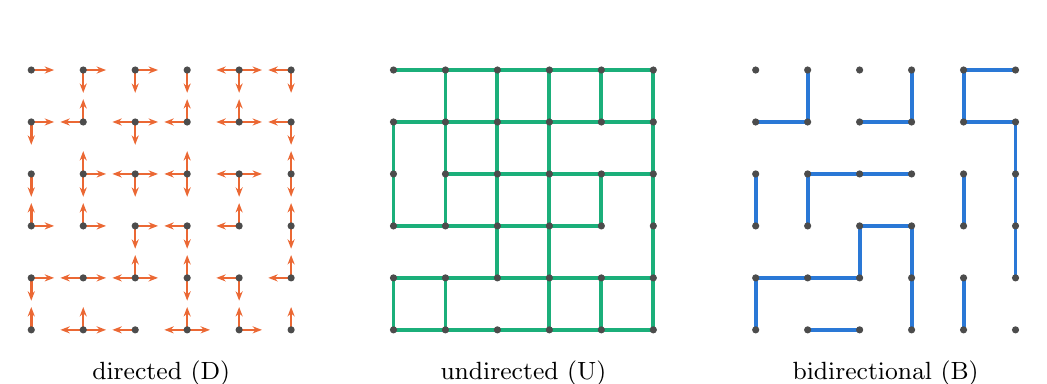
\begin{tikzpicture}
\draw[serD,line width=0.9pt,-{Stealth[length=3.4pt]}] (0.000,0.000)--(0.000,0.290);
\draw[serD,line width=0.9pt,-{Stealth[length=3.4pt]}] (0.000,0.660)--(0.290,0.660);
\draw[serD,line width=0.9pt,-{Stealth[length=3.4pt]}] (0.000,0.660)--(0.000,0.370);
\draw[serD,line width=0.9pt,-{Stealth[length=3.4pt]}] (0.000,1.320)--(0.290,1.320);
\draw[serD,line width=0.9pt,-{Stealth[length=3.4pt]}] (0.000,1.320)--(0.000,1.610);
\draw[serD,line width=0.9pt,-{Stealth[length=3.4pt]}] (0.000,1.980)--(0.000,1.690);
\draw[serD,line width=0.9pt,-{Stealth[length=3.4pt]}] (0.000,2.640)--(0.290,2.640);
\draw[serD,line width=0.9pt,-{Stealth[length=3.4pt]}] (0.000,2.640)--(0.000,2.350);
\draw[serD,line width=0.9pt,-{Stealth[length=3.4pt]}] (0.000,3.300)--(0.290,3.300);
\draw[serD,line width=0.9pt,-{Stealth[length=3.4pt]}] (0.660,0.000)--(0.950,0.000);
\draw[serD,line width=0.9pt,-{Stealth[length=3.4pt]}] (0.660,0.000)--(0.370,0.000);
\draw[serD,line width=0.9pt,-{Stealth[length=3.4pt]}] (0.660,0.000)--(0.660,0.290);
\draw[serD,line width=0.9pt,-{Stealth[length=3.4pt]}] (0.660,0.660)--(0.950,0.660);
\draw[serD,line width=0.9pt,-{Stealth[length=3.4pt]}] (0.660,0.660)--(0.370,0.660);
\draw[serD,line width=0.9pt,-{Stealth[length=3.4pt]}] (0.660,1.320)--(0.950,1.320);
\draw[serD,line width=0.9pt,-{Stealth[length=3.4pt]}] (0.660,1.320)--(0.660,1.610);
\draw[serD,line width=0.9pt,-{Stealth[length=3.4pt]}] (0.660,1.980)--(0.950,1.980);
\draw[serD,line width=0.9pt,-{Stealth[length=3.4pt]}] (0.660,1.980)--(0.660,2.270);
\draw[serD,line width=0.9pt,-{Stealth[length=3.4pt]}] (0.660,1.980)--(0.660,1.690);
\draw[serD,line width=0.9pt,-{Stealth[length=3.4pt]}] (0.660,2.640)--(0.370,2.640);
\draw[serD,line width=0.9pt,-{Stealth[length=3.4pt]}] (0.660,2.640)--(0.660,2.930);
\draw[serD,line width=0.9pt,-{Stealth[length=3.4pt]}] (0.660,3.300)--(0.950,3.300);
\draw[serD,line width=0.9pt,-{Stealth[length=3.4pt]}] (0.660,3.300)--(0.660,3.010);
\draw[serD,line width=0.9pt,-{Stealth[length=3.4pt]}] (1.320,0.000)--(1.030,0.000);
\draw[serD,line width=0.9pt,-{Stealth[length=3.4pt]}] (1.320,0.660)--(1.610,0.660);
\draw[serD,line width=0.9pt,-{Stealth[length=3.4pt]}] (1.320,0.660)--(1.030,0.660);
\draw[serD,line width=0.9pt,-{Stealth[length=3.4pt]}] (1.320,0.660)--(1.320,0.950);
\draw[serD,line width=0.9pt,-{Stealth[length=3.4pt]}] (1.320,1.320)--(1.610,1.320);
\draw[serD,line width=0.9pt,-{Stealth[length=3.4pt]}] (1.320,1.320)--(1.320,1.030);
\draw[serD,line width=0.9pt,-{Stealth[length=3.4pt]}] (1.320,1.980)--(1.610,1.980);
\draw[serD,line width=0.9pt,-{Stealth[length=3.4pt]}] (1.320,1.980)--(1.030,1.980);
\draw[serD,line width=0.9pt,-{Stealth[length=3.4pt]}] (1.320,1.980)--(1.320,1.690);
\draw[serD,line width=0.9pt,-{Stealth[length=3.4pt]}] (1.320,2.640)--(1.610,2.640);
\draw[serD,line width=0.9pt,-{Stealth[length=3.4pt]}] (1.320,2.640)--(1.030,2.640);
\draw[serD,line width=0.9pt,-{Stealth[length=3.4pt]}] (1.320,2.640)--(1.320,2.350);
\draw[serD,line width=0.9pt,-{Stealth[length=3.4pt]}] (1.320,3.300)--(1.610,3.300);
\draw[serD,line width=0.9pt,-{Stealth[length=3.4pt]}] (1.320,3.300)--(1.320,3.010);
\draw[serD,line width=0.9pt,-{Stealth[length=3.4pt]}] (1.980,0.000)--(2.270,0.000);
\draw[serD,line width=0.9pt,-{Stealth[length=3.4pt]}] (1.980,0.000)--(1.690,0.000);
\draw[serD,line width=0.9pt,-{Stealth[length=3.4pt]}] (1.980,0.000)--(1.980,0.290);
\draw[serD,line width=0.9pt,-{Stealth[length=3.4pt]}] (1.980,0.660)--(1.980,0.950);
\draw[serD,line width=0.9pt,-{Stealth[length=3.4pt]}] (1.980,0.660)--(1.980,0.370);
\draw[serD,line width=0.9pt,-{Stealth[length=3.4pt]}] (1.980,1.320)--(1.690,1.320);
\draw[serD,line width=0.9pt,-{Stealth[length=3.4pt]}] (1.980,1.320)--(1.980,1.030);
\draw[serD,line width=0.9pt,-{Stealth[length=3.4pt]}] (1.980,1.980)--(1.690,1.980);
\draw[serD,line width=0.9pt,-{Stealth[length=3.4pt]}] (1.980,1.980)--(1.980,2.270);
\draw[serD,line width=0.9pt,-{Stealth[length=3.4pt]}] (1.980,1.980)--(1.980,1.690);
\draw[serD,line width=0.9pt,-{Stealth[length=3.4pt]}] (1.980,2.640)--(1.690,2.640);
\draw[serD,line width=0.9pt,-{Stealth[length=3.4pt]}] (1.980,2.640)--(1.980,2.930);
\draw[serD,line width=0.9pt,-{Stealth[length=3.4pt]}] (1.980,3.300)--(1.980,3.010);
\draw[serD,line width=0.9pt,-{Stealth[length=3.4pt]}] (2.640,0.000)--(2.930,0.000);
\draw[serD,line width=0.9pt,-{Stealth[length=3.4pt]}] (2.640,0.000)--(2.640,0.290);
\draw[serD,line width=0.9pt,-{Stealth[length=3.4pt]}] (2.640,0.660)--(2.350,0.660);
\draw[serD,line width=0.9pt,-{Stealth[length=3.4pt]}] (2.640,0.660)--(2.640,0.370);
\draw[serD,line width=0.9pt,-{Stealth[length=3.4pt]}] (2.640,1.320)--(2.350,1.320);
\draw[serD,line width=0.9pt,-{Stealth[length=3.4pt]}] (2.640,1.320)--(2.640,1.610);
\draw[serD,line width=0.9pt,-{Stealth[length=3.4pt]}] (2.640,1.980)--(2.930,1.980);
\draw[serD,line width=0.9pt,-{Stealth[length=3.4pt]}] (2.640,1.980)--(2.350,1.980);
\draw[serD,line width=0.9pt,-{Stealth[length=3.4pt]}] (2.640,1.980)--(2.640,1.690);
\draw[serD,line width=0.9pt,-{Stealth[length=3.4pt]}] (2.640,2.640)--(2.930,2.640);
\draw[serD,line width=0.9pt,-{Stealth[length=3.4pt]}] (2.640,2.640)--(2.350,2.640);
\draw[serD,line width=0.9pt,-{Stealth[length=3.4pt]}] (2.640,2.640)--(2.640,2.930);
\draw[serD,line width=0.9pt,-{Stealth[length=3.4pt]}] (2.640,3.300)--(2.930,3.300);
\draw[serD,line width=0.9pt,-{Stealth[length=3.4pt]}] (2.640,3.300)--(2.350,3.300);
\draw[serD,line width=0.9pt,-{Stealth[length=3.4pt]}] (2.640,3.300)--(2.640,3.010);
\draw[serD,line width=0.9pt,-{Stealth[length=3.4pt]}] (3.300,0.000)--(3.300,0.290);
\draw[serD,line width=0.9pt,-{Stealth[length=3.4pt]}] (3.300,0.660)--(3.010,0.660);
\draw[serD,line width=0.9pt,-{Stealth[length=3.4pt]}] (3.300,0.660)--(3.300,0.950);
\draw[serD,line width=0.9pt,-{Stealth[length=3.4pt]}] (3.300,1.320)--(3.300,1.610);
\draw[serD,line width=0.9pt,-{Stealth[length=3.4pt]}] (3.300,1.320)--(3.300,1.030);
\draw[serD,line width=0.9pt,-{Stealth[length=3.4pt]}] (3.300,1.980)--(3.300,2.270);
\draw[serD,line width=0.9pt,-{Stealth[length=3.4pt]}] (3.300,1.980)--(3.300,1.690);
\draw[serD,line width=0.9pt,-{Stealth[length=3.4pt]}] (3.300,2.640)--(3.010,2.640);
\draw[serD,line width=0.9pt,-{Stealth[length=3.4pt]}] (3.300,2.640)--(3.300,2.350);
\draw[serD,line width=0.9pt,-{Stealth[length=3.4pt]}] (3.300,3.300)--(3.010,3.300);
\draw[serD,line width=0.9pt,-{Stealth[length=3.4pt]}] (3.300,3.300)--(3.300,3.010);
\fill[black!70] (0.000,0.000) circle (1.3pt);
\fill[black!70] (0.000,0.660) circle (1.3pt);
\fill[black!70] (0.000,1.320) circle (1.3pt);
\fill[black!70] (0.000,1.980) circle (1.3pt);
\fill[black!70] (0.000,2.640) circle (1.3pt);
\fill[black!70] (0.000,3.300) circle (1.3pt);
\fill[black!70] (0.660,0.000) circle (1.3pt);
\fill[black!70] (0.660,0.660) circle (1.3pt);
\fill[black!70] (0.660,1.320) circle (1.3pt);
\fill[black!70] (0.660,1.980) circle (1.3pt);
\fill[black!70] (0.660,2.640) circle (1.3pt);
\fill[black!70] (0.660,3.300) circle (1.3pt);
\fill[black!70] (1.320,0.000) circle (1.3pt);
\fill[black!70] (1.320,0.660) circle (1.3pt);
\fill[black!70] (1.320,1.320) circle (1.3pt);
\fill[black!70] (1.320,1.980) circle (1.3pt);
\fill[black!70] (1.320,2.640) circle (1.3pt);
\fill[black!70] (1.320,3.300) circle (1.3pt);
\fill[black!70] (1.980,0.000) circle (1.3pt);
\fill[black!70] (1.980,0.660) circle (1.3pt);
\fill[black!70] (1.980,1.320) circle (1.3pt);
\fill[black!70] (1.980,1.980) circle (1.3pt);
\fill[black!70] (1.980,2.640) circle (1.3pt);
\fill[black!70] (1.980,3.300) circle (1.3pt);
\fill[black!70] (2.640,0.000) circle (1.3pt);
\fill[black!70] (2.640,0.660) circle (1.3pt);
\fill[black!70] (2.640,1.320) circle (1.3pt);
\fill[black!70] (2.640,1.980) circle (1.3pt);
\fill[black!70] (2.640,2.640) circle (1.3pt);
\fill[black!70] (2.640,3.300) circle (1.3pt);
\fill[black!70] (3.300,0.000) circle (1.3pt);
\fill[black!70] (3.300,0.660) circle (1.3pt);
\fill[black!70] (3.300,1.320) circle (1.3pt);
\fill[black!70] (3.300,1.980) circle (1.3pt);
\fill[black!70] (3.300,2.640) circle (1.3pt);
\fill[black!70] (3.300,3.300) circle (1.3pt);
\node[font=\small] at (1.650,-0.550) {directed (D)};
\draw[serU,line width=1.4pt] (4.600,0.000)--(5.260,0.000);
\draw[serU,line width=1.4pt] (4.600,0.000)--(4.600,0.660);
\draw[serU,line width=1.4pt] (4.600,0.660)--(5.260,0.660);
\draw[serU,line width=1.4pt] (4.600,1.320)--(5.260,1.320);
\draw[serU,line width=1.4pt] (4.600,1.320)--(4.600,1.980);
\draw[serU,line width=1.4pt] (4.600,1.980)--(4.600,2.640);
\draw[serU,line width=1.4pt] (4.600,2.640)--(5.260,2.640);
\draw[serU,line width=1.4pt] (4.600,3.300)--(5.260,3.300);
\draw[serU,line width=1.4pt] (5.260,0.000)--(5.920,0.000);
\draw[serU,line width=1.4pt] (5.260,0.000)--(5.260,0.660);
\draw[serU,line width=1.4pt] (5.260,0.660)--(5.920,0.660);
\draw[serU,line width=1.4pt] (5.260,1.320)--(5.920,1.320);
\draw[serU,line width=1.4pt] (5.260,1.320)--(5.260,1.980);
\draw[serU,line width=1.4pt] (5.260,1.980)--(5.920,1.980);
\draw[serU,line width=1.4pt] (5.260,1.980)--(5.260,2.640);
\draw[serU,line width=1.4pt] (5.260,2.640)--(5.920,2.640);
\draw[serU,line width=1.4pt] (5.260,2.640)--(5.260,3.300);
\draw[serU,line width=1.4pt] (5.260,3.300)--(5.920,3.300);
\draw[serU,line width=1.4pt] (5.920,0.000)--(6.580,0.000);
\draw[serU,line width=1.4pt] (5.920,0.660)--(6.580,0.660);
\draw[serU,line width=1.4pt] (5.920,0.660)--(5.920,1.320);
\draw[serU,line width=1.4pt] (5.920,1.320)--(6.580,1.320);
\draw[serU,line width=1.4pt] (5.920,1.320)--(5.920,1.980);
\draw[serU,line width=1.4pt] (5.920,1.980)--(6.580,1.980);
\draw[serU,line width=1.4pt] (5.920,1.980)--(5.920,2.640);
\draw[serU,line width=1.4pt] (5.920,2.640)--(6.580,2.640);
\draw[serU,line width=1.4pt] (5.920,2.640)--(5.920,3.300);
\draw[serU,line width=1.4pt] (5.920,3.300)--(6.580,3.300);
\draw[serU,line width=1.4pt] (6.580,0.000)--(7.240,0.000);
\draw[serU,line width=1.4pt] (6.580,0.000)--(6.580,0.660);
\draw[serU,line width=1.4pt] (6.580,0.660)--(7.240,0.660);
\draw[serU,line width=1.4pt] (6.580,0.660)--(6.580,1.320);
\draw[serU,line width=1.4pt] (6.580,1.320)--(7.240,1.320);
\draw[serU,line width=1.4pt] (6.580,1.320)--(6.580,1.980);
\draw[serU,line width=1.4pt] (6.580,1.980)--(7.240,1.980);
\draw[serU,line width=1.4pt] (6.580,1.980)--(6.580,2.640);
\draw[serU,line width=1.4pt] (6.580,2.640)--(7.240,2.640);
\draw[serU,line width=1.4pt] (6.580,2.640)--(6.580,3.300);
\draw[serU,line width=1.4pt] (6.580,3.300)--(7.240,3.300);
\draw[serU,line width=1.4pt] (7.240,0.000)--(7.900,0.000);
\draw[serU,line width=1.4pt] (7.240,0.000)--(7.240,0.660);
\draw[serU,line width=1.4pt] (7.240,0.660)--(7.900,0.660);
\draw[serU,line width=1.4pt] (7.240,1.320)--(7.240,1.980);
\draw[serU,line width=1.4pt] (7.240,1.980)--(7.900,1.980);
\draw[serU,line width=1.4pt] (7.240,2.640)--(7.900,2.640);
\draw[serU,line width=1.4pt] (7.240,2.640)--(7.240,3.300);
\draw[serU,line width=1.4pt] (7.240,3.300)--(7.900,3.300);
\draw[serU,line width=1.4pt] (7.900,0.000)--(7.900,0.660);
\draw[serU,line width=1.4pt] (7.900,0.660)--(7.900,1.320);
\draw[serU,line width=1.4pt] (7.900,1.320)--(7.900,1.980);
\draw[serU,line width=1.4pt] (7.900,1.980)--(7.900,2.640);
\draw[serU,line width=1.4pt] (7.900,2.640)--(7.900,3.300);
\fill[black!70] (4.600,0.000) circle (1.3pt);
\fill[black!70] (4.600,0.660) circle (1.3pt);
\fill[black!70] (4.600,1.320) circle (1.3pt);
\fill[black!70] (4.600,1.980) circle (1.3pt);
\fill[black!70] (4.600,2.640) circle (1.3pt);
\fill[black!70] (4.600,3.300) circle (1.3pt);
\fill[black!70] (5.260,0.000) circle (1.3pt);
\fill[black!70] (5.260,0.660) circle (1.3pt);
\fill[black!70] (5.260,1.320) circle (1.3pt);
\fill[black!70] (5.260,1.980) circle (1.3pt);
\fill[black!70] (5.260,2.640) circle (1.3pt);
\fill[black!70] (5.260,3.300) circle (1.3pt);
\fill[black!70] (5.920,0.000) circle (1.3pt);
\fill[black!70] (5.920,0.660) circle (1.3pt);
\fill[black!70] (5.920,1.320) circle (1.3pt);
\fill[black!70] (5.920,1.980) circle (1.3pt);
\fill[black!70] (5.920,2.640) circle (1.3pt);
\fill[black!70] (5.920,3.300) circle (1.3pt);
\fill[black!70] (6.580,0.000) circle (1.3pt);
\fill[black!70] (6.580,0.660) circle (1.3pt);
\fill[black!70] (6.580,1.320) circle (1.3pt);
\fill[black!70] (6.580,1.980) circle (1.3pt);
\fill[black!70] (6.580,2.640) circle (1.3pt);
\fill[black!70] (6.580,3.300) circle (1.3pt);
\fill[black!70] (7.240,0.000) circle (1.3pt);
\fill[black!70] (7.240,0.660) circle (1.3pt);
\fill[black!70] (7.240,1.320) circle (1.3pt);
\fill[black!70] (7.240,1.980) circle (1.3pt);
\fill[black!70] (7.240,2.640) circle (1.3pt);
\fill[black!70] (7.240,3.300) circle (1.3pt);
\fill[black!70] (7.900,0.000) circle (1.3pt);
\fill[black!70] (7.900,0.660) circle (1.3pt);
\fill[black!70] (7.900,1.320) circle (1.3pt);
\fill[black!70] (7.900,1.980) circle (1.3pt);
\fill[black!70] (7.900,2.640) circle (1.3pt);
\fill[black!70] (7.900,3.300) circle (1.3pt);
\node[font=\small] at (6.250,-0.550) {undirected (U)};
\draw[serB,line width=1.4pt] (9.200,0.000)--(9.200,0.660);
\draw[serB,line width=1.4pt] (9.200,0.660)--(9.860,0.660);
\draw[serB,line width=1.4pt] (9.200,1.320)--(9.200,1.980);
\draw[serB,line width=1.4pt] (9.200,2.640)--(9.860,2.640);
\draw[serB,line width=1.4pt] (9.860,0.000)--(10.520,0.000);
\draw[serB,line width=1.4pt] (9.860,0.660)--(10.520,0.660);
\draw[serB,line width=1.4pt] (9.860,1.320)--(9.860,1.980);
\draw[serB,line width=1.4pt] (9.860,1.980)--(10.520,1.980);
\draw[serB,line width=1.4pt] (9.860,2.640)--(9.860,3.300);
\draw[serB,line width=1.4pt] (10.520,0.660)--(10.520,1.320);
\draw[serB,line width=1.4pt] (10.520,1.320)--(11.180,1.320);
\draw[serB,line width=1.4pt] (10.520,1.980)--(11.180,1.980);
\draw[serB,line width=1.4pt] (10.520,2.640)--(11.180,2.640);
\draw[serB,line width=1.4pt] (11.180,0.000)--(11.180,0.660);
\draw[serB,line width=1.4pt] (11.180,0.660)--(11.180,1.320);
\draw[serB,line width=1.4pt] (11.180,2.640)--(11.180,3.300);
\draw[serB,line width=1.4pt] (11.840,0.000)--(11.840,0.660);
\draw[serB,line width=1.4pt] (11.840,1.320)--(11.840,1.980);
\draw[serB,line width=1.4pt] (11.840,2.640)--(12.500,2.640);
\draw[serB,line width=1.4pt] (11.840,2.640)--(11.840,3.300);
\draw[serB,line width=1.4pt] (11.840,3.300)--(12.500,3.300);
\draw[serB,line width=1.4pt] (12.500,0.660)--(12.500,1.320);
\draw[serB,line width=1.4pt] (12.500,1.320)--(12.500,1.980);
\draw[serB,line width=1.4pt] (12.500,1.980)--(12.500,2.640);
\fill[black!70] (9.200,0.000) circle (1.3pt);
\fill[black!70] (9.200,0.660) circle (1.3pt);
\fill[black!70] (9.200,1.320) circle (1.3pt);
\fill[black!70] (9.200,1.980) circle (1.3pt);
\fill[black!70] (9.200,2.640) circle (1.3pt);
\fill[black!70] (9.200,3.300) circle (1.3pt);
\fill[black!70] (9.860,0.000) circle (1.3pt);
\fill[black!70] (9.860,0.660) circle (1.3pt);
\fill[black!70] (9.860,1.320) circle (1.3pt);
\fill[black!70] (9.860,1.980) circle (1.3pt);
\fill[black!70] (9.860,2.640) circle (1.3pt);
\fill[black!70] (9.860,3.300) circle (1.3pt);
\fill[black!70] (10.520,0.000) circle (1.3pt);
\fill[black!70] (10.520,0.660) circle (1.3pt);
\fill[black!70] (10.520,1.320) circle (1.3pt);
\fill[black!70] (10.520,1.980) circle (1.3pt);
\fill[black!70] (10.520,2.640) circle (1.3pt);
\fill[black!70] (10.520,3.300) circle (1.3pt);
\fill[black!70] (11.180,0.000) circle (1.3pt);
\fill[black!70] (11.180,0.660) circle (1.3pt);
\fill[black!70] (11.180,1.320) circle (1.3pt);
\fill[black!70] (11.180,1.980) circle (1.3pt);
\fill[black!70] (11.180,2.640) circle (1.3pt);
\fill[black!70] (11.180,3.300) circle (1.3pt);
\fill[black!70] (11.840,0.000) circle (1.3pt);
\fill[black!70] (11.840,0.660) circle (1.3pt);
\fill[black!70] (11.840,1.320) circle (1.3pt);
\fill[black!70] (11.840,1.980) circle (1.3pt);
\fill[black!70] (11.840,2.640) circle (1.3pt);
\fill[black!70] (11.840,3.300) circle (1.3pt);
\fill[black!70] (12.500,0.000) circle (1.3pt);
\fill[black!70] (12.500,0.660) circle (1.3pt);
\fill[black!70] (12.500,1.320) circle (1.3pt);
\fill[black!70] (12.500,1.980) circle (1.3pt);
\fill[black!70] (12.500,2.640) circle (1.3pt);
\fill[black!70] (12.500,3.300) circle (1.3pt);
\node[font=\small] at (10.850,-0.550) {bidirectional (B)};
\end{tikzpicture}
\caption{One configuration of the keep sets on a $6\times6$ patch of $\Z^2$ with mean out-degree $\beta=2.5$: every vertex keeps two uniformly chosen directions and, with probability $1/2$, a third one. Left: the directed graph, with an arrow along half of the edge for every kept direction, so that an edge carries two arrows if and only if it is open in the bidirectional graph. Middle: the undirected graph, in which an edge is open if at least one endpoint keeps it. Right: the bidirectional graph, in which an edge is open if both endpoints keep it.}\label{fig:model}
\end{figure}


For $\star\in\{\mathrm B,\mathrm D,\mathrm U\}$ let $\theta^{\star}_d(\beta)$ be the probability that the origin $o$ has an infinite open cluster, respectively an infinite out-cluster in the directed case. In the coupling in which every vertex draws a uniform order of $\cD_d$ and a uniform variable $U_x\in[0,1)$ and keeps the direction in position $i\in\{0,\dots,m-1\}$ if $\beta\ge i+U_x$, the sets $N_x$ increase in~$\beta$. Hence $\theta^{\star}_d$ is non-decreasing, and we define
\begin{equation*}
\bc^{\star}(d)\coloneqq\inf\{\beta\in[0,2d]\colon\theta^{\star}_d(\beta)>0\}\,.
\end{equation*}
Since an open bidirectional path is a directed path and the edges of a directed path are open in the undirected graph,
\begin{equation}\label{eq:order}
\bc^{\mathrm U}(d)\le\bc^{\mathrm D}(d)\le\bc^{\mathrm B}(d)\,.
\end{equation}
In the notation of \cite{BJKLRT25}, $\bc^{\star}(d)=2d\,p^{\star}_{\mathrm c}(d)$. We write $\pc(d)$ for the critical value of Bernoulli bond percolation on $\Z^d$ and $c(d)$ for the connective constant of $\Z^d$. A quantity that appears throughout is
\begin{equation*}
\varphi(\beta)\coloneqq k(k-1+2\varepsilon)=(1-\varepsilon)\,k(k-1)+\varepsilon\,(k+1)k\,,\qquad\beta=k+\varepsilon\,.
\end{equation*}
The probability that a vertex keeps two given edges equals $\varphi(\beta)/(m(m-1))$, whereas a given edge is kept by one endpoint with probability $\beta/m$ and is open in the bidirectional graph with probability $(\beta/m)^2$. The function $\varphi$ is continuous, increasing on $[1,m]$ and linear with slope $2k$ on $[k,k+1]$.

\subsection{Simulations}

We estimated $\bc^{\mathrm B}(d)$ and $\bc^{\mathrm U}(d)$ for $2\le d\le10$ with two methods, both based on the monotone coupling above.
\begin{itemize}
\item \emph{Spanning thresholds} ($d\le4$). For every sample in the box $\{0,\dots,L-1\}^d$ the edges are added in increasing order of the value of $\beta$ at which they become open, and we record the value at which the faces $\{x_1=0\}$ and $\{x_1=L-1\}$ become connected. The empirical distribution functions of this threshold for $L$ and $2L$ cross close to the critical value. In $d=2$ we use $L\in\{512,1024\}$ with $1000$ and $600$ samples; the crossings for $L\in\{64,\dots,1024\}$ agree within $0.002$.
\item \emph{Mean cluster size} ($d\ge3$). On the infinite lattice, with keep sets generated when needed, we estimate the mean size $\chi(\beta)$ of the cluster of the origin from $3000$ samples for a sequence of subcritical $\beta$ with $\chi(\beta)$ up to several hundred or a few thousand, and extrapolate $\chi^{-1/\gamma}$ linearly to zero. We use the exponent $\gamma$ of Bernoulli percolation, $\gamma=1.80,1.44,1.18$ for $d=3,4,5$ and $\gamma=1$ for $d\ge6$.
\end{itemize}
In $d\in\{3,4\}$ both methods agree within $0.0015$. For $d\ge5$ the boxes that can be handled are too small for the first method. For the directed graph we use the values of \cite[Table~1]{CHJK26} for $d\le4$, and for $d\ge5$ the mean size of the out-cluster of the origin with the same extrapolation. The critical exponent of the out-cluster is not known, and in $d\in\{3,4\}$ the extrapolation with the exponents of Bernoulli percolation gives $1.40$ and $1.22$ instead of $1.38$ and $1.20$, so that we expect an uncertainty of about $0.02$ for the directed values. \Cref{tab:sim} and \cref{fig:curves} show the results.

\begin{table}[ht]
\centering
\renewcommand{\arraystretch}{1.15}
\begin{tabular}{cccccccccc}
\toprule
$d$ & 2 & 3 & 4 & 5 & 6 & 7 & 8 & 9 & 10\\
\midrule
$\bc^{\mathrm B}(d)$ & 2.840 & 3.162 & 3.443 & 3.736 & 4.036 & 4.280 & 4.522 & 4.771 & 5.017\\
$\bc^{\mathrm D}(d)$ & 1.84 & 1.38 & 1.20 & 1.146 & 1.109 & 1.088 & 1.074 & 1.064 & 1.057\\
$\bc^{\mathrm U}(d)$ & 1.249 & 1.056 & 1.019 & 1.0093 & 1.0052 & 1.0034 & 1.0025 & 1.0019 & 1.0015\\
\midrule
$\varphi^{-1}(2d)$ & 2.500 & 3.000 & 3.333 & 3.667 & 4.000 & 4.250 & 4.500 & 4.750 & 5.000\\
$1+1/(2d)$ & 1.250 & 1.167 & 1.125 & 1.100 & 1.083 & 1.071 & 1.063 & 1.056 & 1.050\\
$1+1/(8d^2)$ & 1.0313 & 1.0139 & 1.0078 & 1.0050 & 1.0035 & 1.0026 & 1.0020 & 1.0015 & 1.0013\\
\bottomrule
\end{tabular}
\caption{Simulated critical mean out-degrees. For B and U: $d=2$ from the crossing of the spanning-threshold distributions for $L\in\{512,1024\}$, $d\ge3$ from the extrapolation of the mean cluster size; the uncertainty is about $\pm0.005$ for B and $\pm0.001$ for U; for $d\in\{9,10\}$ only the points with $\beta\ge1$ are used for U. For D: \cite[Table~1]{CHJK26} for $d\le4$, and the out-cluster extrapolation for $d\ge5$, with an uncertainty of about $0.02$. The last three rows are the rigorous lower bound for $\bc^{\mathrm B}$ and the leading terms for $\bc^{\mathrm D}$ and $\bc^{\mathrm U}$ from \cref{thm:asymptotics} and \cref{conj:undirected}.}\label{tab:sim}
\end{table}


\begin{figure}[ht]
\centering
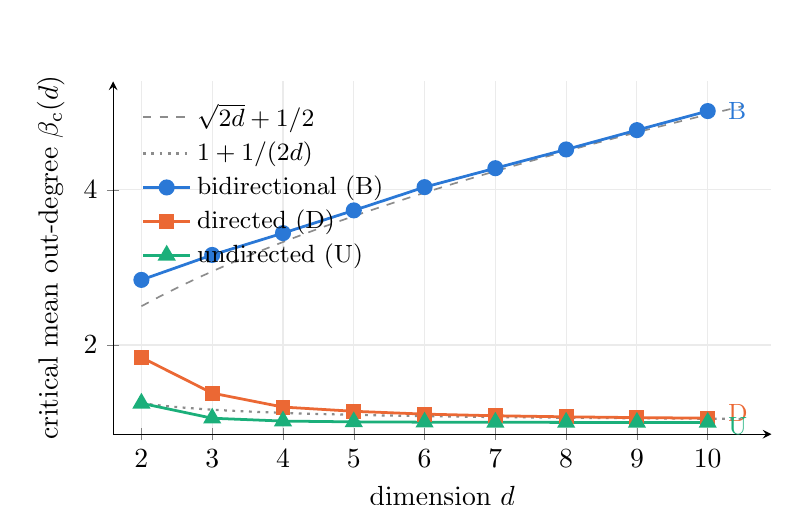
\begin{tikzpicture}
\begin{axis}[width=0.82\textwidth,height=0.5\textwidth,xmin=1.6,xmax=10.9,ymin=0.85,ymax=5.4,
  xlabel={dimension $d$},ylabel={critical mean out-degree $\bc(d)$},xtick={2,...,10},
  axis lines=left,tick style={black!50},grid=major,grid style={black!8},
  every axis plot/.append style={line width=1pt},legend style={draw=none,fill=none,font=\small},legend pos=north west,legend cell align=left]
\addplot[black!45,dashed,domain=2:10.5,samples=60,line width=0.6pt] {sqrt(2*x)+0.5};
\addlegendentry{$\sqrt{2d}+1/2$}
\addplot[black!45,dotted,domain=2:10.5,samples=60,line width=0.8pt] {1+1/(2*x)};
\addlegendentry{$1+1/(2d)$}
\addplot[serB,mark=*,mark size=2.4pt] coordinates {(2,2.8400) (3,3.1617) (4,3.4431) (5,3.7361) (6,4.0361) (7,4.2800) (8,4.5219) (9,4.7711) (10,5.0171)};
\addlegendentry{bidirectional (B)}
\addplot[serD,mark=square*,mark size=2.2pt] coordinates {(2,1.8400) (3,1.3800) (4,1.2000) (5,1.1457) (6,1.1089) (7,1.0880) (8,1.0742) (9,1.0643) (10,1.0568)};
\addlegendentry{directed (D)}
\addplot[serU,mark=triangle*,mark size=2.8pt] coordinates {(2,1.2489) (3,1.0561) (4,1.0192) (5,1.0093) (6,1.0052) (7,1.0034) (8,1.0025) (9,1.0019) (10,1.0015)};
\addlegendentry{undirected (U)}
\node[serB,anchor=west,font=\small] at (axis cs:10.15,5.02) {B};
\node[serD,anchor=west,font=\small] at (axis cs:10.15,1.13) {D};
\node[serU,anchor=west,font=\small] at (axis cs:10.15,0.95) {U};
\end{axis}
\end{tikzpicture}
\caption{Simulated critical mean out-degrees of the bidirectional (circles), directed (squares) and undirected (triangles) lattice neighbour graphs, see \cref{tab:sim}. The dashed and dotted curves are the leading asymptotics of $\bc^{\mathrm B}$ and $\bc^{\mathrm D}$ from \cref{thm:asymptotics}. The uncertainties are smaller than the markers, except for D with $d\ge5$ (about $0.02$).}\label{fig:curves}
\end{figure}


The three curves behave differently. The bidirectional threshold lies only slightly above $\varphi^{-1}(2d)\ge\sqrt{2d}+1/2$, which is a rigorous lower bound (\cref{thm:asymptotics}); the difference is $0.036$, $0.022$ and $0.017$ for $d=6,8,10$. The directed threshold is close to $1+1/(2d)$ already in moderate dimensions. The undirected threshold is much closer to one than the directed one, and $8d^2(\bc^{\mathrm U}(d)-1)$ takes the values $1.9$, $1.5$, $1.3$, $1.3$, $1.2$ and $1.2$ for $d=5,\dots,10$, which suggests that the rigorous lower bound $1+(1+o(1))/(8d^2)$ is sharp.

\subsection{Main results}

The first result compares the three graphs with Bernoulli bond percolation. For $n\in\N$ let $B_n\coloneqq\{x\in\Z^d\colon\|x\|_\infty\le n\}$, $\partial B_n\coloneqq\{x\colon\|x\|_\infty=n\}$, and let $\{o\lra\partial B_n\}$ be the event that $o$ is connected to $\partial B_n$ by an open path in $B_n$ (a directed path in the directed graph). We write $\P^{\star}_{d,\beta}$ for the law of graph $\star$ and $\P^{\bond}_p$ for Bernoulli bond percolation with parameter $p$ on $\Z^d$, and $\theta^{\bond}_d(p)$ for the probability that the open cluster of $o$ is infinite under $\P^{\bond}_p$.

\begin{theorem}\label{thm:comparison}
Let $d\in\N$, $\beta\in[0,2d]$ and $q\coloneqq\sqrt{\varphi(\beta)/(2d(2d-1))}$. Then for all $n\in\N$,
\begin{equation*}
\P^{\mathrm B}_{d,\beta}(o\lra\partial B_n)\ge\P^{\bond}_{q^2}(o\lra\partial B_n)\,,\qquad\P^{\mathrm U}_{d,\beta}(o\lra\partial B_n)\ge\P^{\bond}_{1-(1-q)^2}(o\lra\partial B_n)\,.
\end{equation*}
Moreover, $\P^{\mathrm D}_{d,\beta}(o\lra\partial B_n)\ge\P^{\bond}_{\beta/(2d)}(o\lra\partial B_n)$ \cite[Corollary~3.3, Theorem~2.1 and Lemma~3.5]{BJKLRT25}.
\end{theorem}

The parameter $q$ is optimal: for $|A|=|B|=1$ equality holds in the local inequality behind \cref{thm:comparison}, see \cref{lem:mixture}. Moreover, $q^2\le(\beta/m)^2$, the probability that an edge is open in the bidirectional graph, by \eqref{eq:G1}. The second result gives absence of percolation. For the undirected graph let
\begin{equation*}
\bar\lambda_d(\beta)\coloneqq\frac\beta m-\frac \kappa2+\sqrt \kappa\,,\qquad \kappa\coloneqq\frac{\varphi(\beta)}{m(m-1)}\,.
\end{equation*}

\begin{theorem}\label{thm:absence}
Let $d\ge2$ and $\beta\in[0,2d]$. Then $\theta^{\star}_d(\beta)=0$ in each of the following cases.
\begin{enumerate}
\item[(B)] $\star=\mathrm B$ and $c(d)\,\varphi(\beta)<2d(2d-1)$, in particular if $\varphi(\beta)\le2d$.
\item[(D)] $\star=\mathrm D$ and $c(d)\,\beta<2d$, in particular if $\beta\le2d/(2d-1)$.
\item[(U)] $\star=\mathrm U$ and $\beta\le1$ or $c(d)\,\bar\lambda_d(\beta)<1$.
\end{enumerate}
\end{theorem}

Part (D) is \cite[Lemma~2.2]{CHJK26}, and part (B) extends \cite[Lemma~2.6]{JKLT25} to non-integer~$\beta$. Combined with the known upper bounds on $\pc(d)$ and $c(d)$, \cref{thm:comparison,thm:absence} give explicit bounds in every dimension.

\begin{theorem}\label{thm:bounds}
For every $d\ge2$,
\begin{equation*}
\varphi^{-1}\Big(\frac{2d(2d-1)}{c(d)}\Big)\le\bc^{\mathrm B}(d)\le\varphi^{-1}\big(2d(2d-1)\pc(d)\big)\,,\qquad\frac{2d}{c(d)}\le\bc^{\mathrm D}(d)\le2d\,\pc(d)\,,
\end{equation*}
and $\bc^{\mathrm U}(d)\le\min\{\bc^{\mathrm D}(d),\beta_*\}$, where $\beta_*$ solves $1-(1-q)^2=\pc(d)$ with $q^2=\varphi(\beta_*)/(2d(2d-1))$. With the bounds on $\pc(d)$ and $c(d)$ of \cite{GPS26,FvdH17,PT00}, this gives the values in \cref{tab:bounds}.
\end{theorem}

\begin{table}[ht]
\centering
\begin{tabular}{crrrrrr}
\toprule
$d$ & \multicolumn{2}{c}{$\bc^{\mathrm B}(d)$} & \multicolumn{2}{c}{$\bc^{\mathrm D}(d)$} & \multicolumn{2}{c}{$\bc^{\mathrm U}(d)$}\\
\cmidrule(lr){2-3}\cmidrule(lr){4-5}\cmidrule(lr){6-7}
 & lower & upper & lower & upper & lower & upper\\
\midrule
2 & 2.6197 & $<3$ & 1.4929 & $<2$ & 1.0738 & 1.5148\\
3 & 3.0551 & 3.7365 & 1.2661 & 1.8340 & 1.0252 & 1.5536\\
4 & 3.3717 & 4.4513 & 1.1757 & 1.7110 & 1.0119 & 1.6362\\
5 & 3.6929 & 5.0550 & 1.1286 & 1.6210 & 1.0067 & 1.6210\\
6 & 4.0000 & 5.5358 & 1.0909 & 1.5530 & 1.0035 & 1.5530\\
7 & 4.2500 & 6.0498 & 1.0769 & 1.5120 & 1.0025 & 1.5120\\
8 & 4.5000 & 6.4703 & 1.0666 & 1.4770 & 1.0019 & 1.4770\\
9 & 4.7500 & 6.8804 & 1.0588 & 1.4470 & 1.0015 & 1.4470\\
10 & 5.0000 & 7.2708 & 1.0526 & 1.4220 & 1.0012 & 1.4220\\
11 & 5.2000 & 5.2288 & 1.0476 & 1.0614 & 1.0010 & 1.0614\\
12 & 5.4000 & 5.4206 & 1.0434 & 1.0525 & 1.0008 & 1.0525\\
15 & 6.0000 & 6.0098 & 1.0344 & 1.0386 & 1.0005 & 1.0386\\
20 & 6.8333 & 6.8393 & 1.0256 & 1.0275 & 1.0003 & 1.0275\\
\bottomrule
\end{tabular}
\caption{Rigorous bounds from \cref{thm:absence,thm:bounds,thm:planar,thm:directed}, rounded outwards. For $d=2$ the upper bounds are \cref{thm:planar} and \cite[Theorem~2.3]{CHJK26}. For $d\ge6$ the lower bounds use only $c(d)<2d-1$.}\label{tab:bounds}
\end{table}


\begin{figure}[ht]
\centering
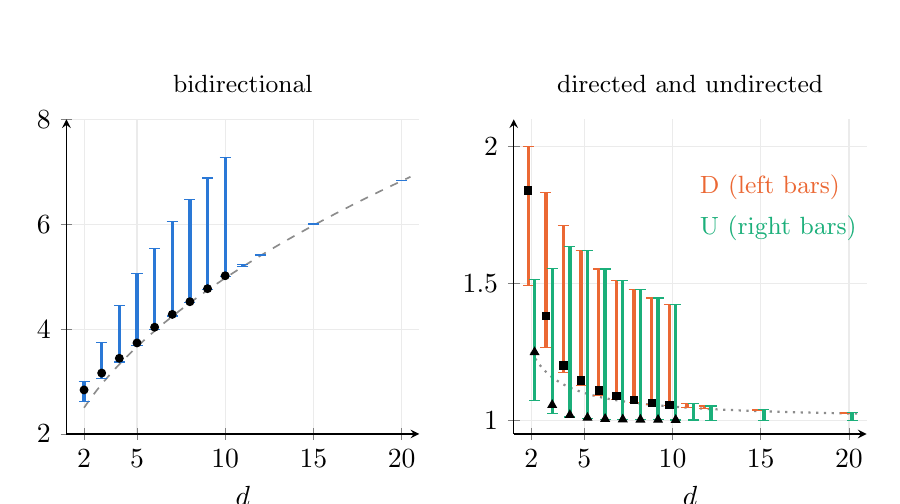
\begin{tikzpicture}
\begin{axis}[name=left,width=0.5\textwidth,height=0.46\textwidth,xmin=1,xmax=21,ymin=2,ymax=8,
  xlabel={$d$},title={\small bidirectional},axis lines=left,tick style={black!50},grid=major,grid style={black!8},
  xtick={2,5,10,15,20}]
\addplot[black!45,dashed,domain=2:20.5,samples=80,line width=0.6pt] {sqrt(2*x)+0.5};
\addplot[serB,draw=none,mark=none,line width=1.2pt,error bars/.cd,y dir=both,y explicit,error mark=-,error bar style={line width=1.2pt,serB}] coordinates {(2,2.8099) +- (0,0.1901) (3,3.3958) +- (0,0.3407) (4,3.9115) +- (0,0.5397) (5,4.3739) +- (0,0.6810) (6,4.7679) +- (0,0.7679) (7,5.1499) +- (0,0.8999) (8,5.4851) +- (0,0.9851) (9,5.8152) +- (0,1.0652) (10,6.1354) +- (0,1.1354) (11,5.2144) +- (0,0.0144) (12,5.4103) +- (0,0.0103) (15,6.0049) +- (0,0.0049) (20,6.8363) +- (0,0.0030)};
\addplot[black,only marks,mark=*,mark size=1.4pt] coordinates {(2,2.8400) (3,3.1617) (4,3.4431) (5,3.7361) (6,4.0361) (7,4.2800) (8,4.5219) (9,4.7711) (10,5.0171)};
\end{axis}
\begin{axis}[at={(left.east)},anchor=west,xshift=1.2cm,width=0.5\textwidth,height=0.46\textwidth,xmin=1,xmax=21,ymin=0.95,ymax=2.1,
  xlabel={$d$},title={\small directed and undirected},axis lines=left,tick style={black!50},grid=major,grid style={black!8},
  xtick={2,5,10,15,20}]
\addplot[black!45,dotted,domain=2:20.5,samples=80,line width=0.8pt] {1+1/(2*x)};
\addplot[serD,draw=none,mark=none,line width=1.2pt,error bars/.cd,y dir=both,y explicit,error mark=-,error bar style={line width=1.2pt,serD}] coordinates {(1.82,1.7465) +- (0,0.2535) (2.82,1.5501) +- (0,0.2839) (3.82,1.4434) +- (0,0.2676) (4.82,1.3748) +- (0,0.2462) (5.82,1.3220) +- (0,0.2310) (6.82,1.2945) +- (0,0.2175) (7.82,1.2718) +- (0,0.2052) (8.82,1.2529) +- (0,0.1941) (9.82,1.2373) +- (0,0.1847) (10.82,1.0545) +- (0,0.0068) (11.82,1.0479) +- (0,0.0045) (14.82,1.0365) +- (0,0.0020) (19.82,1.0266) +- (0,0.0009)};
\addplot[serU,draw=none,mark=none,line width=1.2pt,error bars/.cd,y dir=both,y explicit,error mark=-,error bar style={line width=1.2pt,serU}] coordinates {(2.18,1.2943) +- (0,0.2204) (3.18,1.2894) +- (0,0.2642) (4.18,1.3241) +- (0,0.3121) (5.18,1.3139) +- (0,0.3071) (6.18,1.2783) +- (0,0.2747) (7.18,1.2573) +- (0,0.2547) (8.18,1.2395) +- (0,0.2375) (9.18,1.2243) +- (0,0.2227) (10.18,1.2116) +- (0,0.2104) (11.18,1.0312) +- (0,0.0301) (12.18,1.0266) +- (0,0.0258) (15.18,1.0195) +- (0,0.0190) (20.18,1.0139) +- (0,0.0136)};
\addplot[black,only marks,mark=square*,mark size=1.3pt] coordinates {(1.82,1.84) (2.82,1.38) (3.82,1.2) (4.82,1.1456720535340739) (5.82,1.1088827099348737) (6.82,1.0879819159362831) (7.82,1.074184184089527) (8.82,1.0642669112457324) (9.82,1.056840881486927)};
\addplot[black,only marks,mark=triangle*,mark size=1.7pt] coordinates {(2.18,1.2489) (3.18,1.0561) (4.18,1.0192) (5.18,1.0093) (6.18,1.0052) (7.18,1.0034) (8.18,1.0025) (9.18,1.0019) (10.18,1.0015)};
\node[serD,font=\small,anchor=west] at (axis cs:11,1.85) {D (left bars)};
\node[serU,font=\small,anchor=west] at (axis cs:11,1.7) {U (right bars)};
\end{axis}
\end{tikzpicture}
\caption{Rigorous bounds of \cref{tab:bounds} (vertical bars) and simulated values (black markers) for $d\in\{2,\dots,12,15,20\}$. Left: bidirectional graph with $\sqrt{2d}+1/2$ (dashed). Right: directed (left bars, squares) and undirected (right bars, triangles) graph with $1+1/(2d)$ (dotted). For $d\ge11$ the bounds use the computer-assisted estimates on $\pc(d)$ of \cite{FvdH17}.}\label{fig:bounds}
\end{figure}


The bounds determine the asymptotic behaviour of $\bc^{\mathrm B}$ and $\bc^{\mathrm D}$.

\begin{theorem}\label{thm:asymptotics}
For all $d\ge2$,
\begin{gather*}
\sqrt{2d}+\frac12\le\varphi^{-1}(2d)\le\bc^{\mathrm B}(d)\,,\qquad 1+\frac1{2d-1}\le\bc^{\mathrm D}(d)\,,\\
1+\Big(\frac{\sqrt{2+2/d}-\sqrt2}{2}\Big)^2\le\bc^{\mathrm U}(d)\le\bc^{\mathrm D}(d)\,.
\end{gather*}
Moreover, as $d\to\infty$,
\begin{equation*}
\bc^{\mathrm B}(d)=\varphi^{-1}(2d)+O(d^{-3/2})=\sqrt{2d}+\frac12+O(d^{-1/2})\,,\qquad\bc^{\mathrm D}(d)=1+\frac1{2d}+O(d^{-2})\,,
\end{equation*}
and
\begin{equation*}
1+\frac{1+O(d^{-1})}{8d^2}\le\bc^{\mathrm U}(d)\le1+\frac1{2d}+O(d^{-2})\,.
\end{equation*}
\end{theorem}

In particular, $\bc^{\mathrm D}(d)<\bc^{\mathrm B}(d)$ for all $d\ge2$, since $\bc^{\mathrm D}(d)\le2$ by \cite[Theorem~2.3]{CHJK26} and \cite[Theorem~1.1]{LXZ26}, while $\bc^{\mathrm B}(d)\ge\varphi^{-1}(4)=5/2$. In the plane, the comparison of \cref{thm:comparison} is critical for the bidirectional graph at $\beta=3$, since $\varphi(3)/12=1/2=\pc(2)$. An enhancement argument in the spirit of \cite{AG91}, carried out in \cref{sec:planar}, gives a strict improvement.

\begin{theorem}\label{thm:planar}
$2.6197\le\bc^{\mathrm B}(2)<3$.
\end{theorem}

For the directed graph, \cref{thm:comparison} gives useful upper bounds only in high dimensions, since $2d\,\pc(d)\ge2$ for $3\le d\le10$ with the available bounds on $\pc(d)$. A column projection, which reduces the directed model on $\Z^d$ to a directed model on $\Z^2$ and compares the latter with Bernoulli bond percolation, gives explicit bounds in all dimensions $d\ge3$.

\begin{theorem}\label{thm:directed}
For $3\le d\le30$ we have $\bc^{\mathrm D}(d)\le\bar\beta_d$ with the values $\bar\beta_d$ of \cref{tab:directed}, and $\bc^{\mathrm D}(d)\le1.457$ for all $d\ge31$. In particular,
\begin{equation*}
\sup_{d\ge3}\bc^{\mathrm D}(d)\le1.834\,,\qquad\sup_{d\ge8}\bc^{\mathrm D}(d)\le1.477\,,\qquad\sup_{d\ge9}\bc^{\mathrm D}(d)\le1.457\,.
\end{equation*}
\end{theorem}

\begin{table}[ht]
\centering\small
\setlength{\tabcolsep}{4pt}
\begin{tabular}{l*{10}{c}}
\toprule
$d$ & 3 & 4 & 5 & 6 & 7 & 8 & 9 & 10 & 11 & 12\\
$\bar\beta_d$ & 1.834 & 1.711 & 1.621 & 1.553 & 1.512 & 1.477 & 1.447 & 1.422 & 1.405 & 1.389\\
\midrule
$d$ & 13 & 14 & 15 & 16 & 17 & 18 & 19 & 20 & 21 & 22\\
$\bar\beta_d$ & 1.375 & 1.362 & 1.35 & 1.339 & 1.328 & 1.319 & 1.31 & 1.301 & 1.293 & 1.286\\
\midrule
$d$ & 23 & 24 & 25 & 26 & 27 & 28 & 29 & 30 & ${\ge}31$ & \\
$\bar\beta_d$ & 1.279 & 1.272 & 1.266 & 1.26 & 1.255 & 1.249 & 1.244 & 1.241 & 1.457 & \\
\bottomrule
\end{tabular}
\caption{Rigorous upper bounds $\bar\beta_d$ on $\bc^{\mathrm D}(d)$ from \cref{thm:directed}. For $d\in\{11,\dots,18\}\cup\{20,\dots,24\}$ the bounds $2d\,\pc(d)$ from \cref{thm:comparison}, \cite[Theorem~1.2]{FvdH17} and $\pc(d)\le\pc(15)$, $\pc(d)\le\pc(20)$ are better, see \cref{tab:bounds} for some of them.}\label{tab:directed}
\end{table}

The bound for $d\ge31$ is not obtained by a computation in each dimension. It rests on an algebraic inequality between consecutive dimensions, valid for all mean out-degrees $\beta\in[1.45,2]$ (\cref{lem:consecutive}), which makes a closure-weakened version of the projection bound non-increasing in~$d$. The same method gives the first comparison between two dimensions for the directed graph. By \cref{thm:absence}(D) and $c(2)\le2.679192495$ \cite{PT00} we have
\begin{equation}\label{eq:L2}
\bc^{\mathrm D}(2)\ge4/2.679192495>1.4929\,.
\end{equation}

\begin{theorem}\label{thm:plane}
We have $\bc^{\mathrm D}(7)\le\bc^{\mathrm D}(2)$ and $\bc^{\mathrm D}(d)<\bc^{\mathrm D}(2)$ for all $d\ge8$.
\end{theorem}

For $d\ge8$ this follows from \cref{thm:directed} and \eqref{eq:L2}. The case $d=7$ uses that a five-fold projection of the $7$-dimensional model dominates the planar model locally, for all mean out-degrees between the lower bound \eqref{eq:L2} and $\bar\beta_7$, see the comparison principle in \cref{prop:principle}.

\subsection{Implications for integer \texorpdfstring{$k$}{k}}

For integer $\beta=k$ the model is the lattice $k$-neighbour graph of \cite{JKLT25}. \Cref{tab:integer} updates \cite[Table~1]{BJKLRT25} with what \cref{thm:comparison,thm:absence,thm:planar} give for the bidirectional graph. In $d\in\{2,3\}\cup\{11,\dots,17\}\cup\{20,\dots,23\}$ the integer threshold is determined, and it equals the smallest $k$ with $k(k-1)>2d$. For $2\le d\le10$ this is also the smallest integer above the simulated value of $\bc^{\mathrm B}(d)$. For the directed and the undirected graph the integer threshold is $2$ in every dimension $d\ge2$, so that the continuous parameter is needed to separate the three graphs.

\begin{table}[ht]
\centering
\footnotesize
\setlength{\tabcolsep}{3.5pt}
\renewcommand{\arraystretch}{1.15}
\begin{tabular}{|c|c|c|c|c|c|c|c|}
\hline
\diagbox[width=3.2em,height=2.4em]{$d$}{$k$} & $1$ & $2$ & $3$ & $4$ & $5$ & $6$ & $\ge7$\\\hline
$1$ & no/no/no & yes/yes/yes & -- & -- & -- & -- & --\\\hline
$2$ & no/no/no & no/\cCH{yes}/yes & \cNew{yes}/yes/yes & yes/yes/yes & -- & -- & --\\\hline
$3$ & no/no/no & no/\cLX{yes}/\cLX{yes} & no/\cCH{yes}/yes & \cNew{yes}/yes/yes & yes/yes/yes & yes/yes/yes & --\\\hline
$4$ & no/no/no & no/\cLX{yes}/\cLX{yes} & no/\cBJ{yes}/\cBJ{yes} & open/yes/yes & \cNew{yes}/yes/yes & \cBJ{yes}/yes/yes & yes/yes/yes\\\hline
$5$ & no/no/no & no/\cLX{yes}/\cLX{yes} & no/yes/yes & open/yes/yes & open/yes/yes & \cBJ{yes}/yes/yes & \cBJ{yes}/yes/yes\\\hline
$6$ & no/no/no & no/\cLX{yes}/\cLX{yes} & no/yes/yes & no/yes/yes & open/yes/yes & \cNew{yes}/yes/yes & \cBJ{yes}/yes/yes\\\hline
$7$--$9$ & no/no/no & no/\cLX{yes}/\cLX{yes} & no/yes/yes & no/yes/yes & open/yes/yes & open/yes/yes & \cNew{yes}/yes/yes\\\hline
$10$ & no/no/no & no/\cLX{yes}/\cLX{yes} & no/yes/yes & no/yes/yes & \cNew{no}/yes/yes & open/yes/yes & open/yes/yes\\\hline
$11$--$14$ & no/no/no & no/\cLX{yes}/\cLX{yes} & no/yes/yes & no/yes/yes & \cNew{no}/yes/yes & \cNew{yes}/yes/yes & \cNew{yes}/yes/yes\\\hline
$15$--$17$ & no/no/no & no/\cLX{yes}/\cLX{yes} & no/yes/yes & no/yes/yes & \cNew{no}/yes/yes & \cNew{no}/yes/yes & \cNew{yes}/yes/yes\\\hline
$18$--$19$ & no/no/no & no/\cLX{yes}/\cLX{yes} & no/yes/yes & no/yes/yes & \cNew{no}/yes/yes & \cNew{no}/yes/yes & open/yes/yes\\\hline
$20$ & no/no/no & no/\cLX{yes}/\cLX{yes} & no/yes/yes & no/yes/yes & \cNew{no}/yes/yes & \cNew{no}/yes/yes & \cNew{yes}/yes/yes\\\hline
large & no/no/no & no/\cBJ{yes}/\cBJ{yes} & no/yes/yes & no/yes/yes & no/yes/yes & no/yes/yes & no/yes/yes\\\hline
\end{tabular}
\caption{Percolation results and open cases for the BnG/DnG/UnG with integer $k=\beta$, in the format of \cite[Table~1]{BJKLRT25}. For given $k,d$, ``yes'' means that the given graph percolates, ``no'' that it does not, and ``open'' that the case is at least partially open. Black: \cite{JKLT25}; blue: \cite{CHJK26}; red: \cite{BJKLRT25}; orange: \cite{LXZ26}; green: this paper (\cref{thm:comparison,thm:absence,thm:planar} with the inputs of \cref{tab:bounds}). In the row $7$--$9$ the entry for $k\ge7$ follows for $d=7$ also from \cite[Corollary~3.11]{BJKLRT25} with the bounds of \cite{GPS26}. In $d=10$ and $d\in\{18,19\}$ the BnG percolates for $k\ge8$, and $k=7$ is open in these dimensions. For $d\in\{21,22,23\}$ the BnG percolates if and only if $k\ge8$. The row ``large'' refers to fixed $k$ and all sufficiently large $d$; there the BnG does not percolate as soon as $k(k-1)\le2d$ \cite[Lemma~2.6]{JKLT25}, and by \cref{thm:asymptotics} its critical value of $\beta$ is $\sqrt{2d}+1/2+O(d^{-1/2})$. The red entry for $d=6$, $k\ge7$ follows from \cite[Corollary~3.11]{BJKLRT25} with the bounds of \cite{GPS26}. For $d\ge11$ the green entries use the bounds of \cite[Theorem~1.2]{FvdH17} for $d\in\{11,\dots,15,20\}$, together with $\pc(d)\le\pc(15)$ for $d\in\{16,17\}$ and $\pc(d)\le\pc(20)$ for $d\in\{21,22,23\}$.}\label{tab:integer}
\end{table}


In high dimensions the integer threshold of the bidirectional graph is determined exactly.

\begin{corollary}\label{cor:integer}
There is $d_0\in\N$ such that for all $d\ge d_0$ and $1\le k\le2d$ the bidirectional $k$-neighbour graph on $\Z^d$ percolates if and only if $k(k-1)>2d$. The same equivalence holds for $d\in\{2,3\}\cup\{11,\dots,17\}\cup\{20,\dots,23\}$.
\end{corollary}

The condition has a simple interpretation. Given that the edge $\{x,y\}$ is open, the vertex $y$ keeps each of its other $2d-1$ edges with probability $(k-1)/(2d-1)$, and the corresponding neighbour keeps the edge back with probability $k/(2d)$, so that the expected number of new open edges at $y$ is $k(k-1)/(2d)$. In all cases where percolation of the bidirectional graph is decided, it agrees with this branching heuristic, see \cref{tab:integer}, and so do the simulations for $2\le d\le10$.

\begin{conjecture}\label{conj:integer}
For all $d\ge2$ and $1\le k\le2d$, the bidirectional $k$-neighbour graph on $\Z^d$ percolates if and only if $k(k-1)>2d$.
\end{conjecture}

\begin{remark}\label{rem:integer}
\Cref{conj:integer} replaces \cite[Conjecture~3.3]{JKLT25}, which predicts percolation if and only if $k\ge2\sqrt d$. The \emph{only if} part of that conjecture fails in all sufficiently large dimensions, by \cite[Corollary~3.11]{BJKLRT25} and by \cref{cor:integer}. The first counterexample predicted by \cref{conj:integer} is $(k,d)=(4,5)$, where $4<2\sqrt5$ but $k(k-1)=12>10$; it is supported by the numerical value $\pc(5)\approx0.118$ \cite{MM18}, which lies below $\varphi(4)/(10\cdot9)=2/15$. By \cref{thm:comparison} every open case of \cref{tab:integer} with $k(k-1)>2d$ would follow from a rigorous upper bound on $\pc(d)$, see \cref{tab:open}. Two cases are close: $(k,d)=(5,5)$ and $(6,7)$ require improvements of the bounds of \cite{GPS26} by only $3\%$ and $2\%$.
\end{remark}

\begin{table}[ht]
\centering
\begin{tabular}{cccccc}
\toprule
$d$ & $k$ & $\varphi(k)/(2d(2d-1))$ & bound from \cite{GPS26} & numerical $\pc(d)$ & required improvement\\
\midrule
$4$ & $4$ & $0.2143$ & $0.2788$ & $0.1601$ & $23\%$\\
$5$ & $4$ & $0.1333$ & $0.2284$ & $0.1182$ & $42\%$\\
$5$ & $5$ & $0.2222$ & $0.2284$ & $0.1182$ & $3\%$\\
$6$ & $5$ & $0.1515$ & $0.1922$ & $0.0942$ & $21\%$\\
$7$ & $5$ & $0.1099$ & $0.1682$ & $0.0787$ & $35\%$\\
$7$ & $6$ & $0.1648$ & $0.1682$ & $0.0787$ & $2\%$\\
$8$ & $5$ & $0.0833$ & $0.1486$ & $0.0677$ & $44\%$\\
$8$ & $6$ & $0.1250$ & $0.1486$ & $0.0677$ & $16\%$\\
$9$ & $5$ & $0.0654$ & $0.1326$ & $0.0595$ & $51\%$\\
$9$ & $6$ & $0.0980$ & $0.1326$ & $0.0595$ & $26\%$\\
$10$ & $6$ & $0.0789$ & $0.1206$ & $0.0531$ & $35\%$\\
$10$ & $7$ & $0.1105$ & $0.1206$ & $0.0531$ & $8\%$\\
\bottomrule
\end{tabular}
\caption{Open cases of the bidirectional $k$-neighbour graph for $4\le d\le10$. Each case follows from \cref{thm:comparison} and a rigorous bound $\pc(d)<\varphi(k)/(2d(2d-1))$. The numerical values of $\pc(d)$ are from \cite{MM18}, rounded. The last column is the relative improvement of the bound of \cite{GPS26} needed for this.
}\label{tab:open}
\end{table}

\section{Local comparison}\label{sec:comparison}

\subsection{Pivotal decomposition for both undirected rules}

We treat both undirected graphs at once. Let $\mathrm R\in\{\wedge,\vee\}$, and for a local law $\mu$ on the subsets of $\cD_d$ let $\P^{\mathrm R}_\mu$ be the law of the model in which the sets $N_x$ are i.i.d.\ with law~$\mu$ and $\{x,x+u\}$ is open if $\1\{u\in N_x\}\,\mathrm R\,\1\{-u\in N_{x+u}\}$ holds. Thus $\mathrm R=\wedge$ is the bidirectional and $\mathrm R=\vee$ the undirected graph. For a random set $N$ with law~$\mu$ and $A,B\subseteq\cD_d$ let
\begin{equation*}
\Psi_\mu(A,B)\coloneqq\mu(N\cap A\ne\emptyset,\ N\cap B\neq\emptyset)\,,\qquad\Psi_\mu(A)\coloneqq\mu(N\cap A\neq\emptyset)\,.
\end{equation*}

Fix $n\ge1$ and $a\in B_n$. Let $\cG_a$ be the $\sigma$-algebra generated by $(N_x)_{x\in B_n\setminus\{a\}}$ and let $C_a$ be the event that $o$ is connected to $\partial B_n\setminus\{a\}$ by an open path in $B_n\setminus\{a\}$, with $C_o\coloneqq\emptyset$. Let $O_a$ (resp.\ $T_a$) be the set of $u\in\cD_d$ with $a+u\in B_n$ such that $a+u$ is connected to $o$ (resp.\ to $\partial B_n$) by an open path in $B_n\setminus\{a\}$, and let $O_a^*\subseteq O_a$ and $T_a^*\subseteq T_a$ consist of those $u$ for which $a+u$ keeps the edge to~$a$. All these are $\cG_a$-measurable.

\begin{lemma}\label{lem:pivotal}
Let $a\in B_n\setminus(\{o\}\cup\partial B_n)$. Then $O_a\cap T_a=\emptyset$ on $C_a^\c$, and
\begin{equation*}
\P^{\mathrm R}_\mu(o\lra\partial B_n\,\lvert\,\cG_a)=\1_{C_a}+\1_{C_a^\c}\,\mu(E_a)\,,
\end{equation*}
where, for $\mathrm R=\wedge$, $E_a=\{N\cap O_a^*\neq\emptyset,\,N\cap T_a^*\ne\emptyset\}$, and, for $\mathrm R=\vee$, $E_a=\{O_a^*\neq\emptyset\text{ or }N\cap O_a\neq\emptyset\}\cap\{T^*_a\neq\emptyset\text{ or }N\cap T_a\neq\emptyset\}$. For $a=o$ the same holds with the first condition removed, and for $a\in\partial B_n$ with the second condition removed.
\end{lemma}

\begin{proof}
On $C_a$ the event $\{o\lra\partial B_n\}$ occurs whatever $N_a$ is. On $C_a^\c$, a direction in $O_a\cap T_a$ would connect $o$ to $\partial B_n$ in $B_n\setminus\{a\}$, hence $O_a\cap T_a=\emptyset$. A self-avoiding open path from $o$ to $\partial B_n$ in $B_n$ must visit~$a$; its vertex before $a$ is $a+v$ with $v\in O_a$ and its vertex after $a$ is $a+u$ with $u\in T_a$, and the edges $\{a,a+v\}$ and $\{a,a+u\}$ are open. Conversely, two such open edges give an open path. The edge $\{a,a+u\}$ is open if $u\in N_a$ and $u\in T_a^*\cup O_a^*$ for $\mathrm R=\wedge$, and if $u\in N_a$ or $u\in T_a^*\cup O_a^*$ for $\mathrm R=\vee$. This gives the description of $E_a$, and $N_a$ is independent of $\cG_a$. For $a=o$ only an edge towards $T_o$ is needed, and for $a\in\partial B_n$ only an edge towards $O_a$, since then $a$ itself lies in $\partial B_n$.
\end{proof}

\Cref{fig:pivotal} illustrates the decomposition.

\begin{figure}[ht]
\centering
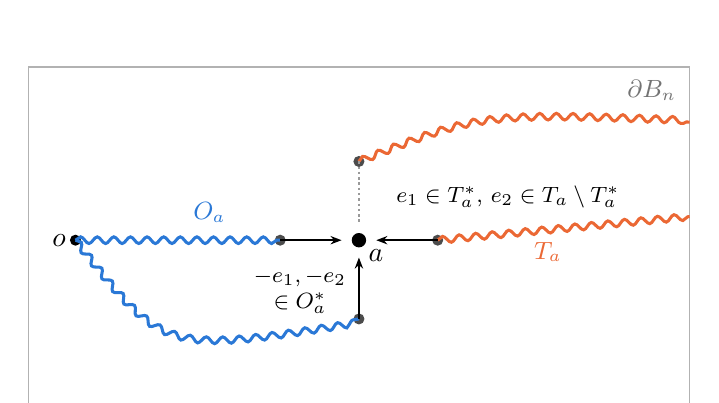
\begin{tikzpicture}[scale=1.0,>={Stealth[length=4pt]}]
\draw[black!30] (-4.2,-2.2) rectangle (4.2,2.2);
\node[black!55,font=\small,anchor=north east] at (4.15,2.15) {$\partial B_n$};
\fill (-3.6,0) circle (2pt) node[left] {$o$};
\fill (0,0) circle (2.6pt) node[below right] {$a$};
\foreach \p/\n in {(-1,0)/w,(0,-1)/s,(1,0)/e,(0,1)/n} \fill[black!70] \p circle (2pt);
\draw[serB,line width=1.1pt,decorate,decoration={snake,amplitude=1.2pt,segment length=6pt}] (-3.6,0)--(-1,0);
\draw[serB,line width=1.1pt,decorate,decoration={snake,amplitude=1.2pt,segment length=6pt}] (-3.6,0) .. controls (-2.5,-1.4) .. (0,-1);
\draw[serD,line width=1.1pt,decorate,decoration={snake,amplitude=1.2pt,segment length=6pt}] (1,0)--(4.2,0.3);
\draw[serD,line width=1.1pt,decorate,decoration={snake,amplitude=1.2pt,segment length=6pt}] (0,1) .. controls (1.5,1.6) .. (4.2,1.5);
\draw[->,black,line width=0.9pt] (-1,0)--(-0.22,0);
\draw[->,black,line width=0.9pt] (0,-1)--(0,-0.22);
\draw[->,black,line width=0.9pt] (1,0)--(0.22,0);
\draw[black!40,densely dotted,line width=0.9pt] (0,1)--(0,0.2);
\node[font=\small,serB] at (-1.9,0.35) {$O_a$};
\node[font=\small,serD] at (2.4,-0.15) {$T_a$};
\node[font=\footnotesize,align=center] at (-0.75,-0.65) {$-e_1,-e_2$\\$\in O_a^*$};
\node[font=\footnotesize,align=left,anchor=west] at (0.35,0.55) {$e_1\in T_a^*$, $e_2\in T_a\setminus T_a^*$};
\end{tikzpicture}
\caption{The pivotal decomposition of \cref{lem:pivotal} at a vertex $a$ that is not already bypassed. The neighbours $a-e_1$ and $a-e_2$ are connected to $o$, and $a+e_1$ and $a+e_2$ to $\partial B_n$, by open paths avoiding $a$, so that $O_a=\{-e_1,-e_2\}$ and $T_a=\{e_1,e_2\}$. Arrows indicate neighbours that keep the edge to $a$; here $O_a^*=\{-e_1,-e_2\}$ and $T_a^*=\{e_1\}$. In the bidirectional graph, $o$ is connected to $\partial B_n$ if and only if $N_a$ meets both $O_a^*$ and $T_a^*$, an event of type $\Psi(A,B)$ with $|A|=1$ and $|B|=2$. In the undirected graph the connection is already present, since $O_a^*$ and $T_a^*$ are nonempty.}\label{fig:pivotal}
\end{figure}


In all cases $\mu(E_a)$ equals $0$, $1$, $\Psi_\mu(A)$ or $\Psi_\mu(A,B)$ for $\cG_a$-measurable sets $A,B$ that are disjoint and nonempty, and the case does not depend on~$\mu$. As in \cite[Theorem~3.9]{BJKLRT25}, replacing the law of one vertex at a time gives the following.

\begin{proposition}\label{prop:l2g}
Let $\mu,\nu$ be local laws such that, for all disjoint nonempty $A,B\subseteq\cD_d$,
\begin{equation}\label{eq:local}
\Psi_\mu(A,B)\ge\Psi_\nu(A,B)\qquad\text{and}\qquad\Psi_\mu(A)\ge\Psi_\nu(A)\,.
\end{equation}
Then $\P^{\mathrm R}_\mu(o\lra\partial B_n)\ge\P^{\mathrm R}_\nu(o\lra\partial B_n)$ for both rules $\mathrm R\in\{\wedge,\vee\}$ and all $n\in\N$.
\end{proposition}

\begin{proof}
Enumerate $B_n=\{a_1,\dots,a_M\}$ and let $\P^{(i)}$ be the law under which $N_{a_1},\dots,N_{a_i}$ have law $\mu$ and the other sets have law~$\nu$. Under $\P^{(i-1)}$ and $\P^{(i)}$ the $\sigma$-algebra $\cG_{a_i}$ has the same law, and by \cref{lem:pivotal} the difference $\P^{(i)}(o\lra\partial B_n)-\P^{(i-1)}(o\lra\partial B_n)$ is the expectation of $\1_{C_{a_i}^\c}$ times $\mu(E_{a_i})-\nu(E_{a_i})$, which is non-negative by \eqref{eq:local}.
\end{proof}

\subsection{The sharp local inequality for mixtures}

Let $\pi_{d,q}$ denote the law of the random set that contains every direction independently with probability~$q$. In the model with local law $\pi_{d,q}$ the edges are independent and open with probability $q^2$ under $\mathrm R=\wedge$ and with probability $1-(1-q)^2$ under $\mathrm R=\vee$.

\begin{lemma}\label{lem:mixture}
Let $d\in\N$, $\beta\in[0,2d]$ and $q\coloneqq\sqrt{\varphi(\beta)/(m(m-1))}$. Then \eqref{eq:local} holds for $\mu=Q_{d,\beta}$ and $\nu=\pi_{d,q}$, with equality in the first inequality if $|A|=|B|=1$.
\end{lemma}

\begin{proof}
Write $\beta=k+\varepsilon$ as above, $u\coloneqq1-q$, $\alpha\coloneqq|A|$ and $\alpha'\coloneqq|B|$. For $0\le j\le m$ and $0\le a\le m$ let $h_j(a)\coloneqq\binom{m-a}{j}/\binom mj$ be the probability that a uniform $j$-subset misses a fixed set of size~$a$, and let $h\coloneqq(1-\varepsilon)h_k+\varepsilon h_{k+1}$. If $\varphi(\beta)=0$, that is $\beta\le1$, then $q=0$, and if $\beta=m$, then $\mu=\pi_{d,1}$; in both cases there is nothing to prove. Let $1<\beta<m$, so that $1\le k\le m-1$ and $\varphi(\beta)>0$. Since $\mu$ and $\nu$ are exchangeable, with $G(a)\coloneqq u^a-h(a)$, inclusion--exclusion gives
\begin{equation*}
\Psi_\mu(A)-\Psi_\nu(A)=G(\alpha)\,,\qquad\Psi_\mu(A,B)-\Psi_\nu(A,B)=G(\alpha)+G(\alpha')-G(\alpha+\alpha')\,.
\end{equation*}
Thus we have to show that $G\ge0$ on $\{0,\dots,m\}$ and that $G$ is subadditive. Let $\Delta(a)\coloneqq G(a+1)-G(a)$.

\emph{Second differences.} Since $h_j(a+1)=h_j(a)(m-a-j)/(m-a)$, a direct computation gives $h_j(a+2)-2h_j(a+1)+h_j(a)=h_j(a)\,j(j-1)/((m-a)(m-a-1))$ for $0\le a\le m-2$. With $q^2=\varphi(\beta)/(m(m-1))$ and $\varphi(\beta)=(1-\varepsilon)k(k-1)+\varepsilon(k+1)k$ we obtain
\begin{equation}\label{eq:second}
\Delta(a+1)-\Delta(a)=q^2\big(u^a-w_1g_k(a)-w_2g_{k+1}(a)\big)\,,\qquad g_j(a)\coloneqq\prod_{i=0}^{a-1}\frac{m-j-i}{m-2-i}\,,
\end{equation}
where $w_1\coloneqq(1-\varepsilon)k(k-1)/\varphi(\beta)$ and $w_2\coloneqq\varepsilon(k+1)k/\varphi(\beta)$ are non-negative with $w_1+w_2=1$. In particular, $\Delta(1)=\Delta(0)$, which is the equality for $|A|=|B|=1$.

\emph{The case $k=1$.} Then $w_1=0$ and $g_2\equiv1$, so that $\Delta(a+1)-\Delta(a)=q^2(u^a-1)\le0$. Hence $G$ is concave with $G(0)=0$, and $G(\alpha+\alpha')-G(\alpha')=\sum_{j<\alpha}\Delta(\alpha'+j)\le\sum_{j<\alpha}\Delta(j)=G(\alpha)$. Moreover, $G(1)\ge0$ by \eqref{eq:G1} below and $G(m)=u^m\ge0$, so that $G\ge0$ by concavity.

\emph{The case $k\ge2$.} Since $g_{k+1}(a)=g_k(a)\,(m-k-a)/(m-k)$, the bracket in \eqref{eq:second} equals $u^a\big(1-r(a)\big)$ with
\begin{equation*}
r(a)\coloneqq u^{-a}g_k(a)\big(1-ca\big)\,,\qquad c\coloneqq\frac{w_2}{m-k}\in\Big[0,\frac1{m-k}\Big]\,.
\end{equation*}
We have $r(0)=1$, and while $r(a)>0$ (which forces $a\le m-k$ and $ca<1$),
\begin{equation*}
\frac{r(a+1)}{r(a)}=\frac1u\Big(1-\frac{k-2}{m-2-a}\Big)\Big(1-\frac{c}{1-ca}\Big)\,.
\end{equation*}
For $a<m-k$ both factors in brackets are positive and non-increasing in~$a$; for $a=m-k$ the first factor vanishes, so that $r(a+1)=0$, and $r$ stays $0$ once it vanishes. Hence $r$ is first non-decreasing and then non-increasing, and $\{a\colon r(a)\ge1\}=\{0,\dots,a_*\}$ for some $0\le a_*\le m-2$. By \eqref{eq:second}, $\Delta$ is non-increasing on $\{0,\dots,a_*+1\}$ and increasing on $\{a_*+1,\dots,m-1\}$. Since $h_j(m-1)=h_j(m)=0$ for $j\ge2$, we have $\Delta(m-1)=-qu^{m-1}<0$, and therefore $\Delta<0$ on $\{a_*+1,\dots,m-1\}$. Let $b\coloneqq\min\{a\colon\Delta(a)\le0\}\le a_*+1$. Then $\Delta(0),\dots,\Delta(b-1)$ are positive and non-increasing, and $\Delta(a)\le0$ for $a\ge b$. Consequently $G$ is non-decreasing with non-increasing increments on $\{0,\dots,b\}$ and non-increasing on $\{b,\dots,m\}$. Since $G(0)=0$ and $G(m)=u^m\ge0$, this gives $G\ge0$. Subadditivity follows: if $\alpha+\alpha'\le b$ use the non-increasing increments; if $\max\{\alpha,\alpha'\}\ge b$ use $G(\alpha+\alpha')\le G(\max\{\alpha,\alpha'\})$ and $G\ge0$; otherwise $G(\alpha+\alpha')\le G(b)\le G(\alpha)+G(b-\alpha)\le G(\alpha)+G(\alpha')$, since $1\le b-\alpha<\alpha'<b$.

\emph{The value $G(1)$.} We have $G(1)=u-h(1)=\beta/m-q$, and
\begin{equation}\label{eq:G1}
(m-1)\beta^2-m\,\varphi(\beta)=k(m-k-2\varepsilon)+(m-1)\varepsilon^2\ge0\,,
\end{equation}
because $m-k-2\varepsilon>0$ for $k\le m-2$ and the left-hand side equals $(m-1)(1-\varepsilon)^2$ for $k=m-1$. Hence $q^2=\varphi(\beta)/(m(m-1))\le(\beta/m)^2$ and $G(1)\ge0$.
\end{proof}

\begin{remark}\label{rem:mixturecheck}
\Cref{lem:mixture} has also been checked numerically in $80$-digit arithmetic for all $m\le40$, all $k$, and seven values of $\varepsilon$, about $2.3\cdot10^6$ pair inequalities, see \texttt{code/check\_mixture\_inequality.py}.
\end{remark}

\begin{proof}[Proof of \cref{thm:comparison}]
Combine \cref{prop:l2g} with \cref{lem:mixture} for both rules. The statement for the directed graph follows from the local inequality \cite[Corollary~3.3]{BJKLRT25}, the local-to-global comparison \cite[Theorem~2.1]{BJKLRT25}, and the identity between directed and undirected Bernoulli one-arm probabilities \cite[Lemma~3.5]{BJKLRT25}, see \cite[Corollary~3.7]{BJKLRT25}.
\end{proof}

\section{Absence of percolation}\label{sec:absence}

We prove \cref{thm:absence} by bounding the expected number of open self-avoiding paths from the origin. For the bidirectional and the directed graph the vertices of a path contribute independent factors; for the undirected graph consecutive edges share a vertex, and a $2\times2$ transfer matrix accounts for this dependence.

\begin{proof}[Proof of \cref{thm:absence}]
Let $c_n(d)$ be the number of self-avoiding paths of length $n$ from~$o$, so that $c_n(d)\le(c(d)+\delta)^n$ for every $\delta>0$ and $n$ large. A self-avoiding path $(x_0,\dots,x_n)$ involves the sets $N_{x_0},\dots,N_{x_n}$ of distinct vertices, which are independent.

(B) The path is open in the bidirectional graph if $x_0$ and $x_n$ keep their path edge and each $x_i$, $0<i<n$, keeps both of its path edges. This has probability $(\beta/m)^2\big(\varphi(\beta)/(m(m-1))\big)^{n-1}$. If $c(d)\varphi(\beta)<m(m-1)$, the expected number of open self-avoiding paths of length $n$ from $o$ tends to zero, and $\theta^{\mathrm B}_d(\beta)=0$. Since $c(d)<2d-1$ for $d\ge2$ \cite[Section~2.3]{JKLT25}, the condition holds if $\varphi(\beta)\le m$.

(D) A directed path is open with probability $(\beta/m)^n$, and the same argument applies, see \cite[Lemma~2.2]{CHJK26}.

(U) For $\beta\le1$ every vertex keeps at most one edge, and the undirected graph is a subgraph of the undirected one-neighbour graph in the coupling of \cref{sec:setting}, which does not percolate by \cite[Proposition~2.5]{JKLT25}. For the second condition, let $f_i\in\{0,1\}$ indicate that $x_i$ keeps the edge $\{x_i,x_{i+1}\}$. The edge $\{x_{i-1},x_i\}$ is open if $f_{i-1}=1$ or $x_i$ keeps $\{x_i,x_{i-1}\}$. For $0<i<n$ the conditional probability, given $f_{i-1}$, that $x_i$ satisfies this requirement and has $f_i=f$ is the entry $(f_{i-1},f)$ of
\begin{equation*}
M\coloneqq\begin{pmatrix}r-\kappa  & \kappa\\1-r&r\end{pmatrix},\qquad r\coloneqq\beta/m\,:
\end{equation*}
if $f_{i-1}=1$ there is no requirement, and if $f_{i-1}=0$ the vertex $x_i$ has to keep the backward edge, which together with the forward edge has probability $\kappa$ and without it $r-\kappa$. Hence the probability that the path is open is at most $\mathbf 1^{\top}M^{n-1}\mathbf 1\le C\lambda^n$ for some $C<\infty$, where
\begin{equation*}
\lambda=r-\frac \kappa2+\sqrt{\kappa\Big(\frac \kappa4+1-r\Big)}\le\bar\lambda_d(\beta)
\end{equation*}
is the Perron root of $M$; the inequality uses $\kappa\le r^2\le4r$, see \eqref{eq:G1}. The claim follows as before.
\end{proof}

\section{Proofs of the main results}\label{sec:proofs}

\begin{proof}[Proof of \cref{thm:bounds}]
The lower bounds are \cref{thm:absence}, and the upper bounds follow from \cref{thm:comparison}, since the comparison models percolate above $\pc(d)$ and $\varphi$ is increasing on $[1,2d]$. For \cref{tab:bounds} we use $\pc(2)=1/2$ \cite{Kes80}; for $3\le d\le10$ the bounds $\pc(d)\le p^*(d)$ of \cite[Theorem~2.1]{GPS26}; the bounds of \cite[Theorem~1.2]{FvdH17} for $d\in\{11,\dots,15,20\}$, together with $\pc(d)\le\pc(d')$ for $d\ge d'$; the bounds $c(2)\le2.679192495$, $c(3)\le4.7387$, $c(4)\le6.8040$, $c(5)\le8.8602$ of \cite{PT00} and $c(d)<2d-1$ otherwise; and for the directed graph also $\bc^{\mathrm D}(d)\le2$ \cite{CHJK26,LXZ26} and the bounds of \cref{thm:directed} for $3\le d\le10$. For the undirected lower bound we use that $\bar\lambda_d$ is increasing on $[1,2d]$, since its derivative is $1/m+\frac12\,\partial_\beta \kappa\,(\kappa^{-1/2}-1)>0$, and solve $c(d)\bar\lambda_d(\beta)=1$ by bisection. See \texttt{code/rigorous\_bounds.py}.
\end{proof}

\begin{proof}[Proof of \cref{cor:integer}]
Let $d\ge2$. If $k(k-1)\le2d$, then $\varphi(k)=k(k-1)\le2d$, and \cref{thm:absence}(B) gives absence of percolation. Conversely, since $k(k-1)$ and $2d$ are even, $k(k-1)>2d$ implies $\varphi(k)\ge2d+2$. As in the proof of \cref{thm:asymptotics} below, $2d(2d-1)\pc(d)\le2d+C/(2d)<2d+2$ for all large $d$, so that \cref{thm:comparison} gives percolation. The explicit dimensions follow from \cref{thm:planar} for $d=2$ and from the bounds of \cref{tab:bounds} and \cite[Theorem~1.2]{FvdH17}, see \cref{tab:integer}; for $d=16,17$ and $d=21,22,23$ we use $\pc(d)\le\pc(15)$ and $\pc(d)\le\pc(20)$, respectively.
\end{proof}

\begin{proof}[Proof of \cref{thm:asymptotics}]
\emph{Bidirectional graph.} By \cref{thm:absence}(B), $\bc^{\mathrm B}(d)\ge\varphi^{-1}(2d)$. Let $k$ be the largest integer with $k(k-1)\le2d$. Then $\varphi^{-1}(2d)=k+(2d-k(k-1))/(2k)=(k+1)/2+d/k$, and with $x_0\coloneqq\sqrt{2d}$,
\begin{equation*}
\varphi^{-1}(2d)-\Big(x_0+\frac12\Big)=\frac{(k-x_0)^2}{2k}\in\Big[0,\frac{1}{2k}\Big]\,,
\end{equation*}
since $|k-x_0|\le1$. This proves the first chain of inequalities and the second equality for $\bc^{\mathrm B}$, once the first is shown. By \cite{HS95} and \cite[Theorem~1.1]{vdHS06}, $\pc(d)=(2d)^{-1}+(2d)^{-2}+O((2d)^{-3})$, so that $m(m-1)\pc(d)\le m+C/m$ for some $C<\infty$ and all large~$d$. On $[k,\infty)$ the function $\varphi$ has slope at least $2k\ge\sqrt{m}$, hence
\begin{equation*}
\bc^{\mathrm B}(d)\le\varphi^{-1}(m+C/m)\le\varphi^{-1}(m)+\frac{C}{m^{3/2}}\,.
\end{equation*}

\emph{Directed graph.} By \cref{thm:absence}(D) and $c(d)<2d-1$, $\bc^{\mathrm D}(d)\ge2d/(2d-1)=1+1/(2d-1)$, and by \cref{thm:comparison}, $\bc^{\mathrm D}(d)\le2d\,\pc(d)=1+1/(2d)+O(d^{-2})$ by \cite{HS95}.

\emph{Undirected graph.} The upper bound follows from \eqref{eq:order}. For the lower bound let $\beta=1+\varepsilon$ with $\varepsilon\in(0,1)$, so that $\varphi(\beta)=2\varepsilon$ and $\kappa=2\varepsilon/(m(m-1))$. Since $c(d)<m-1$,
\begin{equation*}
c(d)\,\bar\lambda_d(\beta)<(m-1)\Big(\frac{1+\varepsilon}m+\sqrt{\frac{2\varepsilon}{m(m-1)}}\Big)\le1-\frac1m+\varepsilon+\sqrt{2\varepsilon}\,,
\end{equation*}
which is at most $1$ if $\varepsilon+\sqrt{2\varepsilon}\le1/m$, that is, if $\sqrt\varepsilon\le(\sqrt{2+4/m}-\sqrt2)/2$. Hence \cref{thm:absence}(U) gives the lower bound, and $((\sqrt{2+2/d}-\sqrt2)/2)^2=(1+O(d^{-1}))/(8d^2)$.
\end{proof}



\section{The directed graph: column projection and comparison of dimensions}\label{sec:column}

In this section we prove \cref{thm:directed,thm:plane}. The method reduces a directed model on $\Z^d$ to a directed model on $\Z^2$ by letting the vertices of a column act together as one vertex of the lattice one dimension lower. It is inspired by the coupling in the proof of \cite[Theorem~2.3]{JKLT25}, and the same reduction was found independently in \cite{LXZ26}, where it is used for $\beta=2$. For a local law $\mu$ on the subsets of $\cD_d$ we write $\P^{\mathrm D}_\mu$ for the directed model, in which every vertex $x$ independently draws $N_x$ with law $\mu$ and sends a directed edge to every $x+u$ with $u\in N_x$, and $\theta^{\mathrm D}_d(\mu)$ for the probability that the out-cluster $\cC(o)$ of the origin is infinite. In particular, $\theta^{\mathrm D}_d(\beta)=\theta^{\mathrm D}_d(Q_{d,\beta})$ in the notation of \cref{sec:setting}.

\subsection{The planar criterion}

For $p\in[0,1]$ the law $\pi_{d,p}$ of \cref{sec:comparison} defines the directed i.i.d.\ model, which has the same one-arm probabilities as Bernoulli bond percolation with parameter~$p$ \cite[Lemma~3.5]{BJKLRT25}. If two local laws satisfy $\mu(N\cap A\neq\emptyset)\le\mu'(N\cap A\neq\emptyset)$ for all nonempty $A\subseteq\cD_d$, then the one-arm probabilities of the directed models satisfy $\P^{\mathrm D}_\mu(o\lra\partial B_n)\le\P^{\mathrm D}_{\mu'}(o\lra\partial B_n)$ for all $n$ \cite[Theorem~2.1]{BJKLRT25}. A law $\nu$ on the subsets of $\cD_d$ is \emph{exchangeable} if it is invariant under all permutations of $\cD_d$. Then $t_\ell\coloneqq\nu(N\cap A=\emptyset)$ depends only on $\ell=\#A$, and we call $t=(t_0,\dots,t_{2d})$ the \emph{avoidance vector} of~$\nu$; it determines~$\nu$.

\begin{lemma}\label{lem:planar}
Let $\nu$ be an exchangeable law on the subsets of $\cD_2$ with avoidance vector $t$. If $t_\ell\le(1-p)^\ell$ for $\ell=1,\dots,4$ and some $p\in(1/2,1]$, then $\theta^{\mathrm D}_2(\nu)\ge\theta^{\bond}_2(p)>0$.
\end{lemma}

\begin{proof}
Since $\pi_{2,p}(N\cap A=\emptyset)=(1-p)^{\#A}$, the assumption is the comparison above for $\mu=\pi_{2,p}$ and $\mu'=\nu$. Together with the identification with bond percolation and \cite{Kes80} this gives the claim.
\end{proof}

\subsection{The column projection}

Let $d\ge3$ and write $x=(y,z)\in\Z^{d-1}\times\Z$. We identify $\cD_{d-1}$ with the horizontal directions in $\cD_d$; the vertical directions are $\pm e_d$. Fix a configuration $(N_x)_{x\in\Z^d}$.

\begin{definition}\label{def:column}
For $y\in\Z^{d-1}$ and $h\in\Z$, the \emph{explored set} $E(y,h)\subseteq\Z$ is the smallest set containing $h$ such that, for every $i\ge0$, the conditions $h+i\in E(y,h)$ and $e_d\in N_{(y,h+i)}$ imply $h+i+1\in E(y,h)$, and the conditions $h-i\in E(y,h)$ and $-e_d\in N_{(y,h-i)}$ imply $h-i-1\in E(y,h)$. The \emph{collected set} is
\begin{equation*}
M(y,h)\coloneqq\bigcup_{z\in E(y,h)}\big(N_{(y,z)}\cap\cD_{d-1}\big)\,.
\end{equation*}
For $u\in M(y,h)$, the \emph{entry height} $\eta(y,h,u)$ is the element $z\in E(y,h)$ with $u\in N_{(y,z)}$ that minimises $|z-h|$, with ties broken towards larger~$z$. The law of $M(y,h)$ is denoted by $\Phi_d(\mu)$.
\end{definition}

The set $E(y,h)$ is an interval containing $h$. Above $h$ it grows as long as the current top vertex keeps $+e_d$, below $h$ as long as the current bottom vertex keeps $-e_d$; a direction pointing back towards $h$ plays no role. Since $M(y,h)$ is a fixed function of the shifted column $(N_{(y,h+z)})_{z\in\Z}$, its law does not depend on $(y,h)$. \Cref{fig:column} shows one step.

\begin{figure}[ht]
\centering
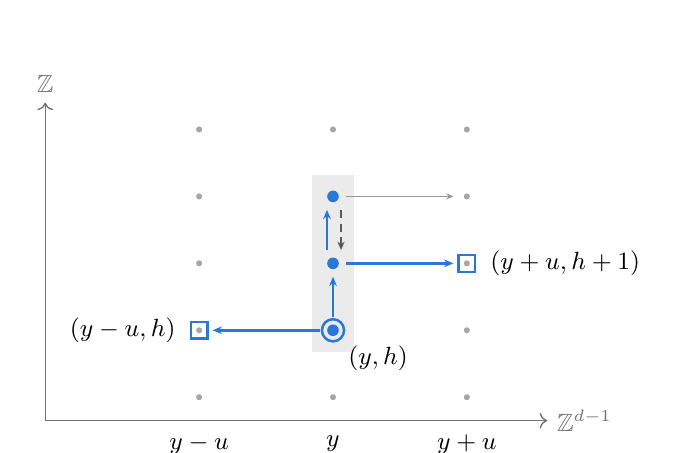
\begin{tikzpicture}[scale=0.85,
  v/.style={circle,fill=black!35,inner sep=0pt,minimum size=2.2pt},
  cv/.style={circle,fill=serB,inner sep=0pt,minimum size=4.2pt},
  orig/.style={circle,draw=serB,line width=0.9pt,inner sep=0pt,minimum size=8pt},
  entry/.style={rectangle,draw=serB,line width=0.8pt,inner sep=0pt,minimum size=6pt},
  edge/.style={-{Stealth[length=2.6pt,width=2.2pt]},black!40,line width=0.45pt},
  clus/.style={-{Stealth[length=3.4pt,width=2.8pt]},serB,line width=0.95pt},
  ign/.style={-{Stealth[length=3pt,width=2.6pt]},black!65,densely dashed,line width=0.6pt},
  guide/.style={black!55,line width=0.5pt}]
\foreach \x in {-2,0,2} \foreach \z in {-1,...,3} \node[v] at (\x,\z) {};
\fill[black!8] (-0.32,-0.32) rectangle (0.32,2.32);
\foreach \z in {0,1,2} \node[cv] at (0,\z) {};
\node[orig] at (0,0) {};
\draw[clus] (0,0.2) -- (0,0.8);
\draw[clus] (-0.2,0) -- (-1.8,0);
\draw[clus] (-0.09,1.2) -- (-0.09,1.8);
\draw[clus] (0.2,1) -- (1.8,1);
\draw[ign] (0.12,1.8) -- (0.12,1.2);
\draw[edge] (0.2,2) -- (1.8,2);
\node[entry] at (-2,0) {};
\node[entry] at (2,1) {};
\node[left=5pt] at (-2,0) {\small $(y-u,h)$};
\node[right=5pt] at (2,1) {\small $(y+u,h+1)$};
\node[below right=2pt] at (0,0) {\small $(y,h)$};
\foreach \x/\l in {-2/{y-u},0/{y},2/{y+u}} \node at (\x,-1.7) {\small $\l$};
\draw[->,guide] (-4.3,-1.35) -- (3.2,-1.35) node[right] {\small $\Z^{d-1}$};
\draw[->,guide] (-4.3,-1.35) -- (-4.3,3.4) node[above] {\small $\Z$};
\end{tikzpicture}
\caption{Schematic column exploration from $(y,h)$; the horizontal axis represents $\Z^{d-1}$ by a single direction~$u$. The vertex $(y,h)$ keeps $+e_d$ and $-u$, the vertex $(y,h+1)$ keeps $+e_d$ and $+u$, and the vertex $(y,h+2)$ keeps $-e_d$, which plays no role (dashed), and $+u$. The explored set (shaded) is $E(y,h)=\{h,h+1,h+2\}$, the collected set is $M(y,h)=\{-u,+u\}$, and the squares mark the entry points $(y-u,h)$ and $(y+u,h+1)$ from which the neighbouring columns are explored.}\label{fig:column}
\end{figure}


\begin{proposition}\label{prop:projection}
For every $d\ge3$ and every local law $\mu$ on the subsets of $\cD_d$ we have $\theta^{\mathrm D}_d(\mu)\ge\theta^{\mathrm D}_{d-1}(\Phi_d(\mu))$.
\end{proposition}

\begin{proof}
Fix an enumeration of $\Z^{d-1}$. We run the following exploration, which maintains a set $D$ of discovered vertices of $\Z^{d-1}$ with heights $h(y)\in\Z$, $y\in D$, and a set $S\subseteq D$ of processed vertices. Initially $D=\{o\}$, $h(o)=0$ and $S=\emptyset$. In step $i\ge1$, if $D\setminus S$ is empty, the exploration stops. Otherwise let $y_i$ be the element of $D\setminus S$ with the smallest index, set $M_i\coloneqq M(y_i,h(y_i))$, add $y_i$ to $S$, and add every $y_i+u$ with $u\in M_i$ and $y_i+u\notin D$ to $D$, with height $h(y_i+u)\coloneqq\eta(y_i,h(y_i),u)$.

\emph{Lifting.} We show that $(y,h(y))\in\cC(o)$ for every $y\in D$, by induction over the order of discovery. This holds for $y=o$. If $y_i+u$ is discovered in step $i$ and $z\coloneqq\eta(y_i,h(y_i),u)$, then $(y_i,h(y_i))$ reaches $(y_i,z)$ along the explored interval, and $(y_i,z)$ has an edge to $(y_i+u,z)=(y_i+u,h(y_i+u))$. Since $y\mapsto(y,h(y))$ is injective, $\#\cC(o)\ge\#D$.

\emph{Law of $D$.} Let $\mathcal F_i$ be the $\sigma$-algebra generated by $y_1,\dots,y_i$ and the sets $N_{(y_l,z)}$, $l\le i$, $z\in\Z$. Whether the exploration stops after step $i$, and otherwise $y_{i+1}$ and $h(y_{i+1})$, are $\mathcal F_i$-measurable. For fixed distinct $z_1,\dots,z_i,y\in\Z^{d-1}$, the event $\{y_1=z_1,\dots,y_i=z_i,\,y_{i+1}=y\}$ depends only on the columns above $z_1,\dots,z_i$, which are independent of the column $\{y\}\times\Z$. Hence, conditionally on $\mathcal F_i$ and on $y_{i+1}=y$, the sets in $\{y\}\times\Z$ are i.i.d.\ with law~$\mu$, and $M_{i+1}$ has law $\Phi_d(\mu)$. By induction over $i$, the sequence $(y_i,M_i)_i$ has the same law as the sequence produced by the same rule from an i.i.d.\ family $(\xi_y)_{y\in\Z^{d-1}}$ with law $\Phi_d(\mu)$, where $\xi_{y_i}$ replaces $M_i$; the heights do not enter the evolution of $D$ and $S$. In the latter exploration every discovered vertex is processed after finitely many steps, and processing $y$ discovers all its out-neighbours $y+\xi_y$. Hence $D$ has the law of the out-cluster of the origin in the directed model on $\Z^{d-1}$ with local law $\Phi_d(\mu)$, and $\P(\#D=\infty)=\theta^{\mathrm D}_{d-1}(\Phi_d(\mu))$. Together with the lifting this proves the claim.
\end{proof}

Applying \cref{prop:projection} successively in dimensions $d,d-1,\dots,3$ gives
\begin{equation}\label{eq:iterate}
\theta^{\mathrm D}_d(\mu)\ge\theta^{\mathrm D}_2\big(\Phi_3\circ\dots\circ\Phi_d(\mu)\big)\,.
\end{equation}

\subsection{The avoidance recursion}

For $j\in\N$ let $\cV_j\coloneqq\{t\in[0,1]^{j+1}\colon 1=t_0>t_1\ge t_2\ge\dots\ge t_j\}$. Avoidance vectors of exchangeable laws with $\nu(N=\emptyset)<1$ lie in $\cV_{2d}$. For $j\ge4$ and $t\in\cV_j$ let $\Gamma(t)_0\coloneqq1$ and, for $1\le\ell\le j-2$,
\begin{equation}\label{eq:Gamma}
\psi_\ell\coloneqq\frac{t_{\ell+1}}{1-t_\ell+t_{\ell+1}}\,,\qquad \Gamma(t)_\ell\coloneqq(1-\psi_\ell)^2\,t_{\ell+2}+2\psi_\ell(1-\psi_\ell)\,t_{\ell+1}+\psi_\ell^2\,t_\ell\,.
\end{equation}
The denominator is at least $1-t_\ell\ge1-t_1>0$.

\begin{lemma}\label{lem:monotone}
Let $j\ge4$. The map $\Gamma$ sends $\cV_j$ to $\cV_{j-2}$, and $t_{\ell+2}\le\Gamma(t)_\ell\le t_\ell$ for $1\le\ell\le j-2$. Moreover, $\Gamma$ is non-decreasing: if $t,t'\in\cV_j$ with $t\le t'$ componentwise, then $\Gamma(t)\le\Gamma(t')$.
\end{lemma}

\begin{proof}
On the set $\mathcal T\coloneqq\{(r_0,r_1,r_2)\colon1>r_0\ge r_1\ge r_2\ge0\}$ let $g(r_0,r_1)\coloneqq r_1/(1-r_0+r_1)$ and $H(r_0,r_1,r_2)\coloneqq(1-g)^2r_2+2g(1-g)r_1+g^2r_0$ with $g=g(r_0,r_1)$, so that $\Gamma(t)_\ell=H(t_\ell,t_{\ell+1},t_{\ell+2})$ for $\ell\ge1$; these triples lie in $\mathcal T$ because $t_\ell\le t_1<1$. The three weights in $H$ are non-negative and sum to one, which gives $r_2\le H\le r_0$. The function $g$ is non-decreasing in $r_0$ and in $r_1$, and
\begin{equation*}
\frac{\partial H}{\partial g}=2(1-g)(r_1-r_2)+2g(r_0-r_1)\ge0\,.
\end{equation*}
Together with the non-negative weights, all partial derivatives of $H$ are non-negative on $\mathcal T$. If $(r_0,r_1,r_2)\le(r_0',r_1',r_2')$ both lie in $\mathcal T$, raising first $r_0$, then $r_1$ and then $r_2$ keeps the triple in $\mathcal T$, so $H(r_0,r_1,r_2)\le H(r_0',r_1',r_2')$. This proves that $\Gamma$ is non-decreasing. Applied to $(t_{\ell+1},t_{\ell+2},t_{\ell+3})\le(t_\ell,t_{\ell+1},t_{\ell+2})$ it gives $\Gamma(t)_{\ell+1}\le\Gamma(t)_\ell$, and $\Gamma(t)_1\le t_1<1$ shows $\Gamma(t)\in\cV_{j-2}$.
\end{proof}

\begin{lemma}\label{lem:recursion}
Let $d\ge3$ and let $\mu$ be an exchangeable law on the subsets of $\cD_d$ with avoidance vector $t\in\cV_{2d}$. Then $\Phi_d(\mu)$ is exchangeable with avoidance vector $\Gamma(t)\in\cV_{2d-2}$.
\end{lemma}

\begin{proof}
The exploration in \cref{def:column} treats all horizontal directions alike, so $\Phi_d(\mu)$ is exchangeable. Fix $A\subseteq\cD_{d-1}$ with $\#A=\ell\in\{1,\dots,2d-2\}$ and consider the exploration from $(o,0)$. Let $\varrho$ be the probability that no vertex $(o,z)$ with $z\ge1$ in $E(o,0)$ keeps a direction in $A$, given that $1\in E(o,0)$; it does not depend on the root. The vertex $(o,1)$ avoids $A\cup\{e_d\}$ with probability $t_{\ell+1}$, and then the exploration stops above; it avoids $A$ and keeps $e_d$ with probability $t_\ell-t_{\ell+1}$, and then the exploration continues from $(o,2)$ with fresh sets; its choice of $-e_d$ plays no role. Hence $\varrho=t_{\ell+1}+(t_\ell-t_{\ell+1})\varrho$, and since $t_\ell-t_{\ell+1}\le t_1<1$, the unique solution is $\varrho=\psi_\ell$. By symmetry the same holds below the root. At the root, exchangeability and inclusion--exclusion show that the probabilities to avoid $A$ and to keep neither, exactly one, or both of $\pm e_d$ are $t_{\ell+2}$, $2(t_{\ell+1}-t_{\ell+2})$ and $t_\ell-2t_{\ell+1}+t_{\ell+2}$. Given the root, the parts above and below are independent, and therefore
\begin{equation*}
\Phi_d(\mu)(N\cap A=\emptyset)=t_{\ell+2}+2(t_{\ell+1}-t_{\ell+2})\,\psi_\ell+(t_\ell-2t_{\ell+1}+t_{\ell+2})\,\psi_\ell^2=\Gamma(t)_\ell\,.
\end{equation*}
For $\ell=0$ both sides equal one, and $\Gamma(t)\in\cV_{2d-2}$ by \cref{lem:monotone}.
\end{proof}

For $\beta\in[1,2]$ the law $Q_{d,\beta}$ is exchangeable with avoidance vector
\begin{equation}\label{eq:tau}
\tau^{(d)}_\ell(\beta)=(2-\beta)\,\frac{2d-\ell}{2d}+(\beta-1)\,\frac{(2d-\ell)(2d-\ell-1)}{2d(2d-1)}\,,\qquad0\le\ell\le2d\,,
\end{equation}
which is non-increasing in $\beta$ for every $\ell$. Since $\Gamma$ is non-decreasing, rounding all entries upwards after each application of $\Gamma$ yields rigorous upper bounds on iterated avoidance vectors; all computer-assisted statements below use exact rational arithmetic with this rounding.

\subsection{Comparison with proper subsets}

The local-to-global comparison of \cite[Theorem~2.1]{BJKLRT25} requires a local inequality for all nonempty sets of directions. Its proof only uses proper subsets, except at the origin, and the origin can be handled separately.

\begin{proposition}\label{prop:proper}
Let $\mu,\nu$ be local laws on the subsets of $\cD_d$ with
\begin{equation}\label{eq:proper}
\mu(N\cap A\ne\emptyset)\le\nu(N\cap A\ne\emptyset)\qquad\text{for all }\emptyset\ne A\subsetneq\cD_d\,.
\end{equation}
If $\theta^{\mathrm D}_d(\mu)>0$, then $\theta^{\mathrm D}_d(\nu)>0$.
\end{proposition}

\begin{proof}
Let $\nu^o$ be the law of the model in which the origin uses $\mu$ and every other vertex uses $\nu$. Fix $n$, and for $U\subseteq B_n\setminus\{o\}$ let $\P^U$ be the law in which the vertices in $U$ use $\nu$ and all others use $\mu$. We show $\P^U(o\lra\partial B_n)\le\P^{U\cup\{a\}}(o\lra\partial B_n)$ for $a\in B_n\setminus(U\cup\{o\})$, where $\lra$ refers to directed paths in $B_n$. Condition on all sets except $N_a$. Either the event $\{o\lra\partial B_n\}$ does not depend on $N_a$, or $o\not\lra\partial B_n$ when $N_a=\emptyset$ while $o\lra a$. In the second case let $A$ be the set of directions $u$ such that $a+u\lra\partial B_n$ without using~$a$; then the event equals $\{N_a\cap A\neq\emptyset\}$, since a path from $o$ to $\partial B_n$ through $a$ leaves $a$ for the last time towards a vertex in $a+A$. Moreover $A\ne\cD_d$: the last vertex $w$ before $a$ on a path from $o$ to $a$ that visits $a$ only at its end satisfies $o\lra w$ without using $a$, so $w-a\in A$ would give $o\lra\partial B_n$ with $N_a=\emptyset$. If $A=\emptyset$, the event fails for every $N_a$. Otherwise \eqref{eq:proper} gives the claim. Adding the vertices of $B_n\setminus\{o\}$ one by one and letting $n\to\infty$ yields $\theta^{\mathrm D}_d(\nu^o)\ge\theta^{\mathrm D}_d(\mu)>0$.

On the event that the out-cluster of $o$ is infinite under $\nu^o$, an infinite self-avoiding path starts with an edge to some $o+u$ and continues without returning to $o$. Writing $G_u$ for the event that $o+u$ has an infinite out-path avoiding~$o$, which depends only on vertices other than $o$ and has the same probability under $\nu^o$ and $\nu$, we obtain $0<\theta^{\mathrm D}_d(\nu^o)\le\sum_u\mu(u\in N)\,\P^{\mathrm D}_\nu(G_u)$. Choose $u$ with $\mu(u\in N)\P^{\mathrm D}_\nu(G_u)>0$. By \eqref{eq:proper} with $A=\{u\}$, $\nu(u\in N)\ge\mu(u\in N)>0$, and independence gives $\theta^{\mathrm D}_d(\nu)\ge\nu(u\in N)\,\P^{\mathrm D}_\nu(G_u)>0$.
\end{proof}

\begin{proposition}[Comparison principle]\label{prop:principle}
Let $d\ge2$, $s\ge1$ and $\beta\in[1,2]$ be such that
\begin{equation}\label{eq:window}
\big(\Gamma^{\circ s}(\tau^{(d+s)}(\beta))\big)_\ell\le\tau^{(d)}_\ell(\beta)\qquad\text{for all }1\le\ell\le2d-1\,.
\end{equation}
If $\theta^{\mathrm D}_d(\beta)>0$, then $\theta^{\mathrm D}_{d+s}(\beta)>0$.
\end{proposition}

\begin{proof}
By \cref{lem:recursion}, $\nu\coloneqq\Phi_{d+1}\circ\dots\circ\Phi_{d+s}(Q_{d+s,\beta})$ is exchangeable with avoidance vector $\Gamma^{\circ s}(\tau^{(d+s)}(\beta))$, and \eqref{eq:window} is exactly \eqref{eq:proper} for $\mu=Q_{d,\beta}$ and this~$\nu$. Hence $\theta^{\mathrm D}_d(\nu)>0$ by \cref{prop:proper}, and \cref{prop:projection}, applied $s$ times, gives $\theta^{\mathrm D}_{d+s}(\beta)\ge\theta^{\mathrm D}_d(\nu)>0$.
\end{proof}

Condition \eqref{eq:window} only involves sets of at most $2d-1$ directions; this is why \cref{prop:proper} is needed.

\subsection{Consecutive dimensions}

\begin{lemma}\label{lem:consecutive}
For all $d\ge3$, $\beta\in[1.45,2]$ and $0\le\ell\le2d-2$ we have $\Gamma(\tau^{(d+1)}(\beta))_\ell\le\tau^{(d)}_\ell(\beta)$.
\end{lemma}

\begin{proof}
Write $\varepsilon\coloneqq\beta-1$, $r\coloneqq2d+2\ge8$ and $a\coloneqq r-\ell\in\{4,\dots,r\}$. For $\ell=0$ both sides equal one, so let $4\le a\le r-1$. Inserting \eqref{eq:tau} into \eqref{eq:Gamma} and simplifying gives
\begin{equation}\label{eq:identity}
\tau^{(d)}_\ell(\beta)-\Gamma(\tau^{(d+1)}(\beta))_\ell=\frac{2(r-a)\,P(a,r,\varepsilon)}{r(r-1)(r-2)(r-3)\,\big((r-1)^2+\varepsilon(r+1-2a)\big)^2}\,,
\end{equation}
where $P$ is a polynomial of degree three in $a$ and in $\varepsilon$ and of degree five in $r$, which the script \texttt{certify\_consecutive\_dimensions.py} prints and checks against \eqref{eq:identity}. The denominator is positive since $(r-1)^2+\varepsilon(r+1-2a)\ge(r-1)^2-(r-3)>0$. It remains to show $P\ge0$. Substitute $\varepsilon=9/20+(11/20)\sigma$ with $\sigma\in[0,1]$ and expand $P$ in the Bernstein basis of degree three in~$\sigma$. On the region $a\ge7$, written as $a=7+x$, $r=8+x+y$ with $x,y\ge0$, and on the three lines $a\in\{4,5,6\}$, $r=8+y$ with $y\ge0$, every Bernstein coefficient is a polynomial in $x,y$ with non-negative coefficients, as verified by computer algebra. These regions cover all pairs $4\le a\le r-1$ with $r\ge8$, so $P\ge0$.
\end{proof}

For $\beta=2$ the polynomial $P$ factorises, and \cref{lem:consecutive} then holds for all $d\ge2$ with a short proof by hand, see also \cite[Lemma~2.4]{LXZ26}. For $\beta=1.3$ the inequality fails in every dimension $3\le d\le300$ that we tested, mostly at $\ell=2d-2$.

The two largest set sizes cannot be compared in this way, because the projected out-set has size at most one with positive probability. We absorb them by a closure: for $t\in\cV_j$ let $(\mathcal Kt)_\ell\coloneqq t_\ell$ for $\ell\le j-2$ and $(\mathcal Kt)_{j-1}=(\mathcal Kt)_j\coloneqq t_{j-2}$, and set
\begin{equation*}
\omega^{(d)}(\beta)\coloneqq(\mathcal K\circ\Gamma)^{\circ(d-2)}\big(\mathcal K\tau^{(d)}(\beta)\big)\in\cV_4\,.
\end{equation*}

\begin{lemma}\label{lem:omega}
Let $\beta\in[1.45,2]$. Then $\Gamma^{\circ(d-2)}(\tau^{(d)}(\beta))\le\omega^{(d)}(\beta)$ for $d\ge3$, and $d\mapsto\omega^{(d)}(\beta)$ is non-increasing on $\{3,4,\dots\}$.
\end{lemma}

\begin{proof}
The first claim follows from $t\le\mathcal Kt$ and the monotonicity of $\Gamma$ and $\mathcal K$. For the second, $\Gamma(\mathcal K\tau^{(d+1)})_\ell=\Gamma(\tau^{(d+1)})_\ell\le\tau^{(d)}_\ell$ for $\ell\le2d-2$ by \cref{lem:consecutive}, since $\mathcal K$ only changes the two largest indices and $\Gamma(t)_\ell$ only depends on $t_\ell,t_{\ell+1},t_{\ell+2}$. As $\mathcal K$ on $\cV_{2d}$ only reads indices up to $2d-2$, this gives $(\mathcal K\circ\Gamma)(\mathcal K\tau^{(d+1)})\le\mathcal K\tau^{(d)}$, and the claim follows by applying the non-decreasing map $(\mathcal K\circ\Gamma)^{\circ(d-2)}$.
\end{proof}

\subsection{Proofs of \texorpdfstring{\cref{thm:directed,thm:plane}}{the results for the directed graph}}

\begin{proof}[Proof of \cref{thm:directed}]
For each pair $(d,\bar\beta_d)$ in \cref{tab:directed} with $d\le30$ we apply $\Gamma$ exactly $d-2$ times to $\tau^{(d)}(\bar\beta_d)$ in rational arithmetic and round every entry upwards to the grid $2^{-100}\Z$ after each step, which keeps the vectors ordered. By \cref{lem:monotone,lem:recursion}, the result bounds the avoidance vector of $\Phi_3\circ\dots\circ\Phi_d(Q_{d,\bar\beta_d})$ from above. In every case its entries satisfy $t_\ell<2^{-\ell}$ for $\ell=1,\dots,4$, see \texttt{code/verify\_uniform\_bounds\_and\_plane.py}, so that \cref{lem:planar} applies with some $p>1/2$, and \eqref{eq:iterate} gives $\theta^{\mathrm D}_d(\bar\beta_d)>0$. By monotonicity in $\beta$, $\bc^{\mathrm D}(d)\le\bar\beta_d$.

For $d\ge31$ let $\beta=1.457$. The upward-rounded vector $\omega^{(31)}(\beta)$ satisfies $t_\ell<2^{-\ell}$ for $\ell=1,\dots,4$, and by \cref{lem:omega}, $\Gamma^{\circ(d-2)}(\tau^{(d)}(\beta))\le\omega^{(d)}(\beta)\le\omega^{(31)}(\beta)$ for every $d\ge31$. As before, $\bc^{\mathrm D}(d)\le1.457$. The suprema follow from the table, since $\bar\beta_d\le1.477$ for $d\ge8$ and $\bar\beta_d\le1.447$ for $9\le d\le30$.
\end{proof}

\begin{proof}[Proof of \cref{thm:plane}]
For $d\ge8$, \cref{thm:directed} and \eqref{eq:L2} give $\bc^{\mathrm D}(d)\le1.477<1.4929\le\bc^{\mathrm D}(2)$. For $d=7$ let $\beta>\bc^{\mathrm D}(2)$. If $\beta\ge\bar\beta_7=1.512$, then $\theta^{\mathrm D}_7(\beta)>0$ by \cref{thm:directed}. Otherwise $\beta\in[1.4929,1.512]$ by \eqref{eq:L2}. Split this interval into $40$ subintervals $[\beta_1,\beta_2]$. Since $\tau^{(d)}(\beta)$ is non-increasing in $\beta$ and $\Gamma$ is monotone, \eqref{eq:window} with $d=2$, $s=5$ holds on $[\beta_1,\beta_2]$ as soon as the upward-rounded vector $\Gamma^{\circ5}(\tau^{(7)}(\beta_1))$ is bounded by the downward-rounded vector $\tau^{(2)}(\beta_2)$ at the indices $\ell\in\{1,2,3\}$, which we verified for every subinterval (\texttt{code/verify\_uniform\_bounds\_and\_plane.py}). \Cref{prop:principle} then gives $\theta^{\mathrm D}_7(\beta)>0$. Hence $\bc^{\mathrm D}(7)\le\bc^{\mathrm D}(2)$.
\end{proof}

\begin{remark}\label{rem:column}
For $\beta=2$ the column projection is the reduction used in \cite{LXZ26} to show that the directed two-neighbour graph percolates in every dimension $d\ge3$, with $\theta^{\mathrm D}_d(2)\ge\theta^{\bond}_2(11/20)$. The obstruction to a direct comparison of consecutive dimensions is discussed in \cref{sec:discussion}.
\end{remark}

\section{The planar bidirectional graph}\label{sec:planar}

In this section $d=2$, and we consider the bidirectional rule $\mathrm R=\wedge$ only. We write $\P_\mu\coloneqq\P^{\wedge}_\mu$, $\cD\coloneqq\cD_2$, $\upsilon\coloneqq\upsilon_{2,3}=Q_{2,3}$, $\pi_q\coloneqq\pi_{2,q}$ and $q_0\coloneqq1/\sqrt2$, so that $\Psi_\upsilon(\{u\},\{v\})=1/2=\Psi_{\pi_{q_0}}(\{u\},\{v\})$ for $u\neq v$.

\subsection{Pivotal vertices and a Russo formula}

In the notation of \cref{lem:pivotal} we call $a\in B_n$ \emph{pivotal} if $T_o^*\neq\emptyset$ (for $a=o$), if $C_a^\c$ occurs and $O_a^*\neq\emptyset$ (for $a\in\partial B_n$), or if $C_a^\c$ occurs and $O_a^*\neq\emptyset\neq T_a^*$ (otherwise). We write $\Piv_a$ for this $\cG_a$-measurable event and
\begin{equation*}
\Xi_\mu(a)\coloneqq\begin{cases}\Psi_\mu(T_o^*)&\text{if }a=o\,,\\\Psi_\mu(O_a^*)&\text{if }a\in\partial B_n\,,\\\Psi_\mu(T_a^*,O_a^*)&\text{otherwise}\,.\end{cases}
\end{equation*}
By \cref{lem:pivotal}, $\P_\mu(o\lra\partial B_n\,\lvert\,\cG_a)=\1_{C_a}+\1_{\Piv_a}\Xi_\mu(a)$, since $\mu(E_a)=0$ on $C_a^\c\setminus\Piv_a$. The pair $(T_a^*,O_a^*)$, or the single set $T_o^*$ or $O_a^*$, is the \emph{type} of a pivotal vertex.

\begin{lemma}\label{lem:russo}
Let $\lambda\mapsto\mu_\lambda$ be a family of local laws such that $\lambda\mapsto\mu_\lambda(S)$ is differentiable for every $S\subseteq\cD$, and write $\partial_\lambda\Xi_{\mu_\lambda}(a)$ for the derivative of $\lambda\mapsto\Xi_{\mu_\lambda}(a)$ at a fixed type. Then, for every $n\in\N$,
\begin{equation*}
\frac{\d}{\d \lambda}\P_{\mu_\lambda}(o\lra\partial B_n)=\sum_{a\in B_n}\E_{\mu_\lambda}\big[\1_{\Piv_a}\,\partial_\lambda\Xi_{\mu_\lambda}(a)\big]\,.
\end{equation*}
\end{lemma}

\begin{proof}
The probability is a finite sum of products $\prod_{x\in B_n}\mu_\lambda(S_x)$ over configurations $(S_x)_{x\in B_n}$ in $E\coloneqq\{o\lra\partial B_n\}$. By the product rule, the term for $a$ equals $\E_{\mu_\lambda}\big[\sum_{S}\partial_\lambda\mu_\lambda(S)\,\1_{E}\big((N_x)_{x\ne a},S\big)\big]$, where $((N_x)_{x\ne a},S)$ denotes the configuration with $N_a$ replaced by $S$. By \cref{lem:pivotal} the inner sum equals $\1_{C_a}\partial_\lambda\sum_S\mu_\lambda(S)+\1_{\Piv_a}\partial_\lambda\Xi_{\mu_\lambda}(a)$, and the first term vanishes because $\sum_S\mu_\lambda(S)=1$.
\end{proof}

\subsection{Strategy}

For $q,t\in[0,1]$ let
\begin{equation*}
\mu_{q,t}\coloneqq(1-t)\,\pi_q+t\,\upsilon\,,\qquad f_n(q,t)\coloneqq\P_{\mu_{q,t}}(o\lra\partial B_n)\,.
\end{equation*}
The function $f_n$ is a polynomial in $(q,t)$, and $f_n(q,0)$ is the corresponding probability for Bernoulli bond percolation with parameter $q^2$. The idea is to compare the effect of the two parameters on $f_n$. By \cref{lem:russo}, both partial derivatives are sums over pivotal vertices. Increasing $t$ replaces the product law by the uniform law. Near $q=q_0$ this helps strictly at every pivotal vertex except at those of type $(\{u\},\{v\})$ (\cref{lem:differences}), at which it is neutral for $q=q_0$ by \cref{lem:mixture}. We call these pivotal vertices \emph{tight}. A local surgery shows that tight pivotal vertices are, up to a constant, not more likely than non-tight ones (\cref{lem:surgery}). This yields a differential inequality $\partial_tf_n\ge\gamma\,\partial_qf_n$ near $(q_0,0)$ with $\gamma>0$ independent of $n$ (\cref{lem:differential}). Integrating it along a line of slope $-\gamma$ as in \cite{AG91} shows that a supercritical bond percolation is dominated by a model $\mu_{q',t}$ with $q'<q_0$ (\cref{prop:enhanced}). Finally, $Q_{2,3-\delta'}$ dominates $\mu_{q',t}$ in the sense of \eqref{eq:local} for small $\delta'>0$.

\subsection{The local differences}

For a pivotal vertex $a$ let $\Delta_q(a)\coloneqq\Xi_\upsilon(a)-\Xi_{\pi_q}(a)$. A pivotal vertex $a\in B_n\setminus(\{o\}\cup\partial B_n)$ is \emph{tight} if $|T_a^*|=|O_a^*|=1$; all other pivotal vertices, including all pivotal vertices in $\{o\}\cup\partial B_n$, are \emph{non-tight}. We write $\Piv_a^{\mathrm t}$ and $\Piv_a^{\mathrm{nt}}$ for the corresponding events, both $\cG_a$-measurable.

\begin{lemma}\label{lem:differences}
Let $|q-q_0|\le\delta\le1/1600$. On $\Piv_a^{\mathrm{nt}}$ we have $\Delta_q(a)\ge1/400$, and on $\Piv_a^{\mathrm t}$ we have $\Delta_q(a)\ge-2\delta$. Moreover, $0\le\partial_q\Xi_{\pi_q}(a)\le4$ on $\Piv_a$, and $\Delta_{q_0}(a)\ge1/200$ on $\Piv_a^{\mathrm{nt}}$.
\end{lemma}

\begin{proof}
For an increasing event of the four independent indicators of $\pi_q$, Russo's formula gives $0\le\partial_q\pi_q(\cdot)\le4$. This proves the third claim and shows that $q\mapsto\Xi_{\pi_q}(a)$ is $4$-Lipschitz. Since $\upsilon$ is the law of $\cD\setminus\{R\}$ with $R$ uniform on~$\cD$, the non-tight types have the following values, where $i=|A|$ and $j=|B|$:
\begin{equation*}
\Psi_\upsilon(A)=\begin{cases}3/4&i=1\,,\\1&i\ge2\,,\end{cases}\qquad\Psi_\upsilon(A,B)=\begin{cases}3/4&\min\{i,j\}=1<\max\{i,j\}\,,\\1&i=j=2\,.\end{cases}
\end{equation*}
With $r\coloneqq1-q_0$, the corresponding values of $\pi_{q_0}$ are $1-r^i$ and $(1-r^i)(1-r^j)$. The differences $\Delta_{q_0}$ are $3/4-q_0\approx0.0429$, $r^2\approx0.0858$, $r^3\approx0.0251$, $r^4\approx0.0074$ for the single sets, and $3/4-q_0(1-r^2)\approx0.1036$, $3/4-q_0(1-r^3)\approx0.0607$, $1-(1-r^2)^2\approx0.1642$ for the pairs; see \texttt{code/local\_differences\_planar.py}. All are at least $r^4\ge1/200$, and by the Lipschitz property $\Delta_q(a)\ge1/200-4\delta\ge1/400$ on $\Piv^{\mathrm{nt}}_a$. On $\Piv_a^{\mathrm t}$ we have $\Delta_q(a)=1/2-q^2\ge1/2-(q_0+\delta)^2=-2q_0\delta-\delta^2\ge-2\delta$.
\end{proof}

\subsection{The surgery}

For $a\in\Z^2$ let $\Lambda_a\coloneqq(a+\{-2,\dots,2\}^2)\cap B_n$. Then $\#\Lambda_a\le25$, and every vertex lies in at most $25$ of the sets $\Lambda_a$.

\begin{lemma}\label{lem:surgery}
Let $n\ge5$, $q\in[3/5,4/5]$, $t\in[0,1/2]$ and $m_0\coloneqq1/1250$. Then for every $a\in B_n\setminus(\{o\}\cup\partial B_n)$,
\begin{equation*}
\P_{\mu_{q,t}}(\Piv_a)\le m_0^{-25}\sum_{a'\in\Lambda_a}\P_{\mu_{q,t}}(\Piv^{\mathrm{nt}}_{a'})\,.
\end{equation*}
\end{lemma}

\begin{proof}
Write $\Lambda\coloneqq\Lambda_a$, let $\omega_{\mathrm{out}}\coloneqq(N_x)_{x\in B_n\setminus\Lambda}$, and let $G_{\mathrm{out}}$ be the graph on $B_n\setminus\Lambda$ formed by the open edges with both endpoints outside~$\Lambda$; it is a function of $\omega_{\mathrm{out}}$. Every set $S\subseteq\cD$ satisfies $\mu_{q,t}(S)\ge(1-t)\min\{q,1-q\}^4\ge\frac12\cdot5^{-4}=m_0$.

\emph{Reduction.} Let $F$ be the set of outside configurations $\omega_{\mathrm{out}}$ for which some choice of $(N_x)_{x\in\Lambda}$ makes $a$ pivotal. Since $\Piv_a$ does not depend on $N_a$, $\Piv_a\subseteq\{\omega_{\mathrm{out}}\in F\}$. We show below that there is a map $\xi$, assigning to every $\omega_{\mathrm{out}}\in F$ a choice $\xi(\omega_{\mathrm{out}})=(S_x)_{x\in\Lambda}$, such that the configuration $(\omega_{\mathrm{out}},\xi(\omega_{\mathrm{out}}))$ lies in $\Piv_{a'}^{\mathrm{nt}}$ for some $a'\in\Lambda$. Then, by independence,
\begin{equation*}
\sum_{a'\in\Lambda}\P(\Piv^{\mathrm{nt}}_{a'})\ge\P\big(\omega_{\mathrm{out}}\in F,\ (N_x)_{x\in\Lambda}=\xi(\omega_{\mathrm{out}})\big)\ge m_0^{\#\Lambda}\,\P(\omega_{\mathrm{out}}\in F)\ge m_0^{25}\,\P(\Piv_a)\,.
\end{equation*}

\emph{Ports.} Fix $\omega_{\mathrm{out}}\in F$ and a completion making $a$ pivotal; we may set $N_a=\cD$, since this does not affect $\Piv_a$. Then $o\lra\partial B_n$ by \cref{lem:pivotal}, and every open path from $o$ to $\partial B_n$ in $B_n$ visits $a$, since $C_a$ fails. In particular, $o$ and $\partial B_n$ are not connected in $G_{\mathrm{out}}$, a subgraph of the open graph without~$a$. Let $\pi=(\pi_0,\dots,\pi_\ell)$ be a self-avoiding open path from $o$ to $\partial B_n$ in $B_n$ that visits $\partial B_n$ only at its end. It visits $a$, which is neither $o$ nor in $\partial B_n$. We call a pair $(x,y)$ with $x\in\Lambda$, $y\in B_n\setminus\Lambda$, $|x-y|=1$ and $x-y\in N_y$ an \emph{$o$-port} if $y$ is connected to $o$ in $G_{\mathrm{out}}$, and a \emph{$\partial$-port} if $y$ is connected to $\partial B_n$ in $G_{\mathrm{out}}$. These notions depend only on $\omega_{\mathrm{out}}$. If $o\notin\Lambda$, no pair is both, since $o$ and $\partial B_n$ are not connected in $G_{\mathrm{out}}$, and the outside vertex of an $o$-port is not in $\partial B_n$. In each of the three cases below, $\xi(\omega_{\mathrm{out}})$ is defined from the lexicographically first ports with the required properties and from a deterministic construction, so that it depends on $\omega_{\mathrm{out}}$ only. In every case all vertices of $\Lambda$ outside an explicit subgraph $H$ keep no edge, and the vertices of $H$ keep exactly the edges listed. Then the open edges with at least one endpoint in $\Lambda$ are exactly the listed edges.

\emph{Case 1: $3\le\|a\|_\infty\le n-3$.} Then $o\notin\Lambda$ and $\Lambda=a+\{-2,\dots,2\}^2\subseteq B_{n-1}$. Let $i_1\coloneqq\min\{i\colon\pi_{i+1}\in\Lambda\}$ and $i_2\coloneqq\max\{i\colon\pi_{i-1}\in\Lambda\}$. The pieces $(\pi_0,\dots,\pi_{i_1})$ and $(\pi_{i_2},\dots,\pi_\ell)$ lie in $G_{\mathrm{out}}$, so that $(\pi_{i_1+1},\pi_{i_1})$ is an $o$-port and $(\pi_{i_2-1},\pi_{i_2})$ is a $\partial$-port. Moreover $\pi_{i_1+1}\neq\pi_{i_2-1}$, since otherwise $\pi$ would meet $\Lambda$ in a single vertex, which would have to be~$a$, while $a$ has no neighbour outside~$\Lambda$. Hence there are an $o$-port $(x_1,y_1)$ and a $\partial$-port $(x_2,y_2)$ with $x_1\neq x_2$, and we take the lexicographically first such pair; both $x_1,x_2$ lie on the ring $R\coloneqq\{x\colon\|x-a\|_\infty=2\}$, which is a cycle of $16$ vertices.

The gadget consists of the square $a$, $a+e_1$, $a+e_1+e_2$, $a+e_2$ and four spokes, see \cref{fig:surgery}: the two \emph{$a$-spokes} $(a-2e_1,a-e_1)$ and $(a-2e_2,a-e_2)$, which end next to $a$, and the two \emph{$c$-spokes} $(a+2e_1+e_2)$ and $(a+e_1+2e_2)$, which end next to $c\coloneqq a+e_1+e_2$. The spokes are pairwise disjoint, disjoint from the square, and each meets $R$ exactly in its first vertex, its \emph{end}. In the cyclic order of $R$ the ends appear as $a+2e_1+e_2$, $a+e_1+2e_2$, $a-2e_1$, $a-2e_2$, so that the two ends of each kind are adjacent in this order.

We claim that there are disjoint paths $P_1$ from $x_1$ to an end $s_1$ and $P_2$ from $x_2$ to an end $s_2$, both within $R$, such that $s_1$ and $s_2$ are of different kinds. Cut $R$ at $x_1$ and $x_2$ into two arcs $\rho,\rho'$, each containing $x_1$ and $x_2$. If one arc, say $\rho$, contains ends of both kinds, let $s_1$ be the first end on $\rho$ seen from $x_1$ and $s_2$ an end of the other kind on~$\rho$; then $s_2$ comes after $s_1$, and the sub-arcs from $x_1$ to $s_1$ and from $s_2$ to $x_2$ are disjoint. Otherwise each arc contains ends of one kind only, and since all four ends lie in $\rho\cup\rho'$, both arcs contain ends, of different kinds. Let $P_1$ run along $\rho$ from $x_1$ to its first end and $P_2$ along $\rho'$ from $x_2$ to its first end. These paths are disjoint: they could only meet in $x_1$ or $x_2$, which would then be an end lying on both arcs, contradicting that the arcs carry different kinds.

Let $H$ be the graph whose edges are the edges between consecutive vertices of $P_1$, of $P_2$ and of the spokes at $s_1$ and $s_2$, the edge between the last vertex of the $a$-spoke and $a$, the edge between the last vertex of the $c$-spoke and $c$, and the four edges of the square. Every vertex of $H$ keeps exactly its edges in $H$; in addition $x_1$ keeps $\{x_1,y_1\}$ and $x_2$ keeps $\{x_2,y_2\}$. All other vertices of $\Lambda$ keep nothing. Then the open edges meeting $\Lambda$ are the edges of $H$ together with $\{x_1,y_1\}$ and $\{x_2,y_2\}$: they form a path from $y_1$ through $P_1$ and the spoke at $s_1$ to the square, the square, and a path from the square through the spoke at $s_2$ and $P_2$ to~$y_2$.

Consider the new configuration and $a'\coloneqq a$. Removing $a$ splits the open edges meeting $\Lambda$ into a piece attached to $y_1$ and a piece attached to $y_2$. The piece attached to $y_1$ contains no vertex of $\partial B_n$, because $\Lambda\cap\partial B_n=\emptyset$, and in $G_{\mathrm{out}}$ the cluster of $o$ contains $y_1$ but no vertex of $\partial B_n$ and not $y_2$. Hence $C_a$ fails. If $s_1$ is an $a$-end, then $O_a^*$ consists of the direction of the last vertex of the spoke at $s_1$, and $T_a^*=\{e_1,e_2\}$; if $s_1$ is a $c$-end, then $O_a^*=\{e_1,e_2\}$ and $T_a^*$ consists of the direction of the last vertex of the spoke at $s_2$. The remaining neighbour of $a$ keeps nothing. In both cases $a$ is pivotal with $\{|T_a^*|,|O_a^*|\}=\{1,2\}$, hence non-tight.

\emph{Case 2: $\|a\|_\infty\le2$.} Then $o\in\Lambda$, $\Lambda\subseteq B_4$, and $\Lambda\cap\partial B_n=\emptyset$ since $n\ge5$. With $i_2$ as in Case~1 there is a $\partial$-port, and we take the lexicographically first one, $(x_2,y_2)$. Let $H$ be a shortest path in the box $\Lambda$ from $o$ to $x_2$; its vertices keep the edges along $H$, and $x_2$ also keeps $\{x_2,y_2\}$. Then the neighbour of $o$ on $H\cup\{y_2\}$ keeps the edge to $o$ and is connected to $\partial B_n$ without using~$o$, so that $T_o^*\ne\emptyset$, and the origin is pivotal, which is non-tight by definition.

\emph{Case 3: $n-2\le\|a\|_\infty\le n-1$.} Then $o\notin\Lambda$ because $n\ge5$, and $\Lambda$ is a box meeting $\partial B_n$. With $i_1$ as in Case~1 we see that an $o$-port exists, and we take the lexicographically first one, $(x_1,y_1)$; then $y_1\notin\partial B_n$. Let $H$ be a shortest path in $\Lambda$ from $x_1$ to $\Lambda\cap\partial B_n$, ending at $z$; only its last vertex lies in $\partial B_n$, and $H=\{x_1\}$ if $x_1\in\partial B_n$. The vertices of $H$ keep the edges along $H$, and $x_1$ also keeps $\{x_1,y_1\}$. Removing $z$, the open edges meeting $\Lambda$ form a path from $y_1$ that contains no vertex of $\partial B_n$, and the cluster of $o$ in $G_{\mathrm{out}}$ contains no vertex of $\partial B_n$. Hence $C_z$ fails, the neighbour of $z$ on $H\cup\{y_1\}$ gives a direction in $O_z^*$, and $z\in\partial B_n$ is pivotal, hence non-tight.

The three cases cover all $a\in B_n\setminus(\{o\}\cup\partial B_n)$, since $n-2\ge3$.
\end{proof}

\begin{figure}[ht]
\centering
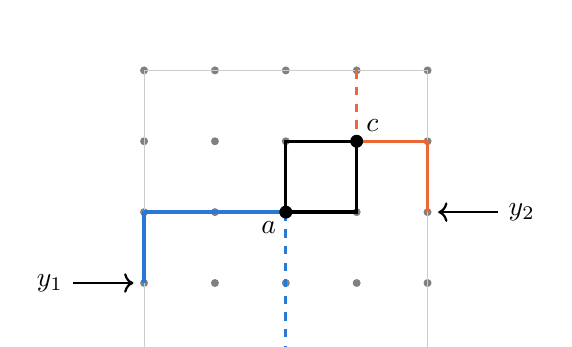
\begin{tikzpicture}[scale=0.9]
\foreach \x in {-2,...,2} \foreach \y in {-2,...,2} \fill[black!50] (\x,\y) circle (1.6pt);
\draw[black!20] (-2,-2) rectangle (2,2);
\draw[very thick] (0,0)--(1,0)--(1,1)--(0,1)--cycle;
\draw[very thick,serB] (-2,0)--(0,0);
\draw[very thick,serB,dashed] (0,-2)--(0,0);
\draw[very thick,serD] (2,1)--(1,1);
\draw[very thick,serD,dashed] (1,2)--(1,1);
\fill (0,0) circle (2.6pt) node[below left] {$a$};
\fill (1,1) circle (2.6pt) node[above right] {$c$};
\draw[thick,->] (-3,-1)--(-2.15,-1) node[pos=0,left] {$y_1$};
\draw[very thick,serB] (-2,-1)--(-2,0);
\draw[thick,->] (3,0)--(2.15,0) node[pos=0,right] {$y_2$};
\draw[very thick,serD] (2,0)--(2,1);
\end{tikzpicture}
\caption{The surgery of Case~1 in the proof of \cref{lem:surgery} in the box $a+\{-2,\dots,2\}^2$. The $a$-spokes are drawn in blue, the $c$-spokes in orange; one spoke of each kind (solid) is used. Here $x_1=a-2e_1-e_2$ is connected to the $a$-end $a-2e_1$ and $x_2=a+2e_1$ to the $c$-end $a+2e_1+e_2$ along the ring. After the surgery $a$ is pivotal with $|T_a^*|=2$ and $|O_a^*|=1$.}\label{fig:surgery}
\end{figure}

\subsection{The differential inequality and the proof of \texorpdfstring{\cref{thm:planar}}{the planar upper bound}}

Let $K\coloneqq25\,m_0^{-25}$, $\delta\coloneqq1/(1600K)$ and $\gamma\coloneqq1/(3200(1+K))$.

\begin{lemma}\label{lem:differential}
For all $n\ge5$, $q\in[q_0-\delta,q_0+\delta]$ and $t\in[0,1/2]$,
\begin{equation*}
\partial_tf_n(q,t)\ge\gamma\,\partial_qf_n(q,t)\ge0\,.
\end{equation*}
\end{lemma}

\begin{proof}
Write $\P=\P_{\mu_{q,t}}$ and $S_{\mathrm t}\coloneqq\sum_{a\in B_n}\P(\Piv^{\mathrm t}_a)$, $S_{\mathrm{nt}}\coloneqq\sum_{a\in B_n}\P(\Piv^{\mathrm{nt}}_a)$. Since $\partial_t\mu_{q,t}=\upsilon-\pi_q$ and $\partial_q\mu_{q,t}=(1-t)\partial_q\pi_q$, \cref{lem:russo} and \cref{lem:differences} give
\begin{equation*}
\partial_tf_n=\sum_{a\in B_n}\E\big[\1_{\Piv_a}\Delta_q(a)\big]\ge\frac{S_{\mathrm{nt}}}{400}-2\delta S_{\mathrm t}\,,\qquad 0\le\partial_qf_n\le4\,(S_{\mathrm t}+S_{\mathrm{nt}})\,.
\end{equation*}
Since $q\in[3/5,4/5]$, \cref{lem:surgery} applies, and since every $a'$ lies in at most $25$ of the sets $\Lambda_a$, it gives $S_{\mathrm t}\le K S_{\mathrm{nt}}$. Hence $\partial_tf_n\ge(1/400-2\delta K)S_{\mathrm{nt}}=S_{\mathrm{nt}}/800$ and $\partial_qf_n\le4(1+K)S_{\mathrm{nt}}$, which gives the claim.
\end{proof}

\begin{proposition}\label{prop:enhanced}
Let $t\coloneqq1/2$. There is $q'<q_0$ such that the bidirectional model with local law $\mu_{q',t}$ percolates.
\end{proposition}

\begin{proof}
Let $q_1\coloneqq q_0+\gamma/4$, $q'\coloneqq q_0-\gamma/4$ and $g_n(\lambda)\coloneqq f_n(q_1-\gamma\lambda,\lambda)$ for $\lambda\in[0,1/2]$. Along this segment $|q_1-\gamma\lambda-q_0|\le\gamma/4\le\delta$, so that \cref{lem:differential} gives $g_n'(\lambda)=\partial_tf_n-\gamma\,\partial_qf_n\ge0$ for $n\ge5$. Hence
\begin{equation*}
f_n(q',t)=g_n(t)\ge g_n(0)=f_n(q_1,0)=\P^{\bond}_{q_1^2}(o\lra\partial B_n)\ge\theta^{\bond}_2(q_1^2)
\end{equation*}
for all $n\ge5$, where $\theta^{\bond}_2$ is the percolation probability of Bernoulli bond percolation on $\Z^2$. Since $q_1^2>1/2$, the right-hand side is positive by \cite{Kes80}, and letting $n\to\infty$ gives the claim.
\end{proof}

\begin{proof}[Proof of \cref{thm:planar}]
The lower bound is \cref{tab:bounds}. For the upper bound let $t=1/2$ and $q'$ be as in \cref{prop:enhanced}. We show that $Q_{2,3-\delta'}=(1-\delta')\upsilon+\delta'\upsilon_{2,2}$ satisfies \eqref{eq:local} with respect to $\mu_{q',t}$ for small $\delta'>0$. For every type $T$ (a pair $(A,B)$ or a single set $A$),
\begin{equation*}
\Psi_{Q_{2,3-\delta'}}(T)-\Psi_{\mu_{q',t}}(T)=(1-t)\big(\Psi_\upsilon(T)-\Psi_{\pi_{q'}}(T)\big)-\delta'\big(\Psi_\upsilon(T)-\Psi_{\upsilon_{2,2}}(T)\big)\,.
\end{equation*}
The first term is at least $\eta\coloneqq(1-t)\min\{1/2-q'^2,1/200\}>0$: for $|A|=|B|=1$ it equals $(1-t)(1/2-q'^2)$, and for all other types $\Psi_\upsilon-\Psi_{\pi_{q'}}\ge\Psi_\upsilon-\Psi_{\pi_{q_0}}\ge1/200$ by \cref{lem:differences}. The second term is at most $\delta'$. Hence \eqref{eq:local} holds for $\delta'\le\eta$, and \cref{prop:l2g} together with \cref{prop:enhanced} gives $\theta^{\mathrm B}_2(3-\delta')>0$.
\end{proof}

\section{Discussion}\label{sec:discussion}

\emph{The undirected graph.} The rigorous upper bound $\bc^{\mathrm U}(d)\le\bc^{\mathrm D}(d)\le1+1/(2d)+O(d^{-2})$ is far from the simulated values, while the lower bound of \cref{thm:asymptotics} is close to them, see \cref{tab:sim}.

\begin{conjecture}\label{conj:undirected}
$\bc^{\mathrm U}(d)=1+(1+o(1))/(8d^2)$ as $d\to\infty$.
\end{conjecture}

The lower bound comes from counting self-avoiding paths, which is asymptotically sharp for many high-dimensional models. A matching upper bound requires a comparison that does not pass through the directed graph. The comparison of \cref{thm:comparison} with Bernoulli bond percolation of parameter $1-(1-q)^2\approx2q$ only gives $\bc^{\mathrm U}(d)\le1+1/8+o(1)$, since it loses the information that every vertex keeps at least one edge. At $\beta=1$ the undirected graph is the undirected one-neighbour graph, which does not percolate \cite[Proposition~2.5]{JKLT25}, and \cref{thm:asymptotics} shows that a positive density of vertices with two kept edges is needed in every dimension. The strict inequality $\bc^{\mathrm U}(d)<\bc^{\mathrm D}(d)$, which the simulations show with a large margin, is open in every dimension.

\emph{The bidirectional graph.} For $d\ge11$ the bounds of \cref{tab:bounds} determine $\bc^{\mathrm B}(d)$ within $0.03$, and for $3\le d\le10$ the upper bounds are limited by the available rigorous bounds on $\pc(d)$. The simulations suggest $\bc^{\mathrm B}(d)-\varphi^{-1}(2d)\approx0.53\,d^{-3/2}$, in line with the order of the error term in \cref{thm:asymptotics}. For $2\le d\le8$ the simulated values lie strictly below the comparison value $\varphi^{-1}(2d(2d-1)\pc(d))$ evaluated with the numerical estimates of $\pc(d)$ of \cite{MM18}, by margins between $0.16$ ($d=2$) and $0.009$ ($d=8$); for instance $\bc^{\mathrm B}(6)\approx4.036<4.054$. For $d\in\{9,10\}$ the margins are within the statistical errors. As for $d=2$ (\cref{thm:planar}), we expect that an enhancement argument gives this strict inequality in general.

\emph{The directed graph.} \Cref{thm:asymptotics} determines $\bc^{\mathrm D}(d)$ up to $O(d^{-2})$. More precisely, $c(d)<2d-1$ and the expansion $\pc(d)=(2d)^{-1}+(2d)^{-2}+\frac72(2d)^{-3}+O(d^{-4})$ of \cite{HS95,vdHS06} give $\bc^{\mathrm D}(d)=1+(2d)^{-1}+a_d(2d)^{-2}$ with $1+o(1)\le a_d\le\frac72+o(1)$.
The bounds of \cref{tab:directed} decrease in $d$ for $d\le30$, and the simulations suggest the following, in line with \cite[Conjecture~3.2]{JKLT25}.

\begin{conjecture}\label{conj:monotone}
The map $d\mapsto\bc^{\mathrm D}(d)$ is strictly decreasing.
\end{conjecture}

In contrast to $\pc(d)$, which decreases because $\Z^d$ embeds into $\Z^{d+1}$, the mean out-degree is fixed when the dimension grows, so that the additional neighbours dilute the choices, and no inclusion argument is available. For Bernoulli bond percolation, the expansion of $\pc(d)$ in \cite{HS95,vdHS06} shows that $d\mapsto2d\,\pc(d)$ is strictly decreasing for all sufficiently large~$d$, with a threshold that is not explicit; as far as we know, monotonicity in low dimensions, including the first step $4\pc(2)>6\pc(3)$, is open there as well.
If \eqref{eq:window} held with $s=1$ for all $\beta$ in a neighbourhood of $\bc^{\mathrm D}(d)$, then \cref{prop:principle} would give $\bc^{\mathrm D}(d+1)\le\bc^{\mathrm D}(d)$, that is, the non-strict version of \cref{conj:monotone}. For $d\in\{2,3\}$ the set of $\beta\in[1,2]$ for which \eqref{eq:window} holds with $s=1$ is empty: at $\ell=2d-1$ the difference of the two sides is a rational function of $\beta$ without zeros in $[1,2]$ and of the wrong sign. For larger $d$ we computed these sets on a grid, with endpoints accurate to within $0.005$: $[1.69,1.89]$ for $d=4$, $[1.59,1.96]$ for $d=6$ and $[1.55,1.99]$ for $d=10$ (\texttt{code/obstruction\_intervals.py}). These intervals lie above the simulated critical values. With more projection steps they grow: for $d=2$ they are approximately $[1.62,1.91]$, $[1.52,1.96]$ and $[1.45,1.98]$ for $s=3,4,5$, and $[1.30,2.00]$ for $s=10$. The difference $\tau^{(d)}_\ell(\beta)-\Gamma(\tau^{(d+1)}(\beta))_\ell$ is positive for small $\ell$, since the column collects on average more than $\beta$ horizontal directions, and negative for $\ell$ close to $2d$, because the projected out-set is empty or a single direction with a probability that a degree-constrained law cannot match; for instance, for $d=2$ and $\beta=1.84$ the differences are $0.042$, $0.020$, $-0.009$ for $\ell=1,2,3$.

We see four routes towards \cref{conj:monotone}. First, \cref{prop:principle} with $s=4$ gives $\bc^{\mathrm D}(6)\le\bc^{\mathrm D}(2)$ as soon as $\bc^{\mathrm D}(2)\ge1.52$ is known rigorously, and any rigorous improvement of \eqref{eq:L2} translates into new comparisons. Second, interpolating between $Q_{d,\beta}$ and the projected law site by site, the derivative of the one-arm probability is a sum over pivotal vertices of the local differences above; the negative contributions come from pivotal vertices whose set of good directions is almost all of $\cD_d$, and a local modification of a neighbour could trade them against the gains at small $\ell$. Third, richer explorations than single columns, for instance of whole fibres, collect more choices, but an exactly computable version is needed. Fourth, for $\beta=2$ \cref{lem:consecutive} holds for all $d\ge2$, and whether $\theta^{\mathrm D}_d(2)$ itself is non-decreasing in $d$ is open.

\emph{Monotonicity in the dimension.} The simulations suggest that $\bc^{\mathrm U}$ and $\bc^{\mathrm D}$ are decreasing and $\bc^{\mathrm B}$ is increasing in~$d$, and that $\bc^{\mathrm B}(d)-\varphi^{-1}(2d)$ is decreasing. None of these statements is proved. The intervals of \cref{tab:bounds} for $d\in\{11,12,15,20\}$ are disjoint and increasing, so that at least $\bc^{\mathrm B}(11)<\bc^{\mathrm B}(12)<\bc^{\mathrm B}(15)<\bc^{\mathrm B}(20)$.

\emph{Planar values.} In the plane, $\bc^{\mathrm B}(2)\approx2.840$, $\bc^{\mathrm D}(2)\approx1.84$ and $\bc^{\mathrm U}(2)\approx1.249$. We are not aware of an exact solution or a duality relation for any of them. Since the discarded sets $\cD_2\setminus N_x$ have law $Q_{2,4-\beta}$, the closed edges of the undirected graph form a bidirectional graph of the discarded sets, but on the primal rather than the dual lattice, so that planar duality does not apply directly.


\section*{Acknowledgements}
The author acknowledges the financial support of the Leibniz Association within the Leibniz Junior Research Group on Probabilistic Methods for Dynamic Communication Networks (DYCOMNET) as part of the Leibniz Competition (grant no.\ J105/2020), of the Berlin Mathematics Research Center MATH+ through the project EF-MA-Sys-2 on Information Flow \& Emergent Behavior in Complex Networks, and of the Deutsche Forschungsgemeinschaft (DFG) through Project P27 within the SPP~2265.

\section*{Use of AI tools}
The simulations, proofs, computations and the text of this note were developed with substantial assistance of the AI system Claude (Anthropic), in an interactive process directed by the author.

\section*{Code}
{\raggedright The code is available from the author on request and in the GitHub repository \url{https://github.com/jonaskoeppl/percolation-discrete-knn}. The simulations use the C programs \texttt{sim\_spanning\_thresholds.c} (spanning thresholds in boxes) and \texttt{sim\_mean\_cluster\_size.c} (mean cluster size on the infinite lattice), with \texttt{run\_spanning\_simulations.sh} as driver; the raw output is in \texttt{simulation\_data.tar.gz}. The Python scripts are the following.
\begin{itemize}
\item \texttt{estimate\_from\_spanning.py}: crossing points of the spanning-threshold distributions with bootstrap errors ($d\le4$).
\item \texttt{cluster\_size\_fit\_bidirectional.py}, \texttt{cluster\_size\_fit\_undirected.py}, \texttt{cluster\_size\_fit\_directed.py}: adaptive choice of $\beta$, mean cluster sizes and extrapolation of $\chi^{-1/\gamma}$ for the three graphs ($d\ge3$).
\item \texttt{rigorous\_bounds.py}: the bounds of \cref{tab:bounds}, from the published bounds on $\pc(d)$ and $c(d)$, in exact rational arithmetic.
\item \texttt{make\_tables\_and\_figures.py}: generates \cref{tab:sim,tab:bounds} and \cref{fig:curves,fig:bounds}.
\item \texttt{make\_model\_figure.py}: generates \cref{fig:model}.
\item \texttt{check\_mixture\_inequality.py}: numerical check of \cref{lem:mixture}, see \cref{rem:mixturecheck}.
\item \texttt{local\_differences\_planar.py}: the local differences in \cref{lem:differences}.
\item \texttt{verify\_uniform\_bounds\_and\_plane.py}: certification of \cref{thm:directed,thm:plane} in exact rational arithmetic.
\item \texttt{certify\_consecutive\_dimensions.py}: the identity \eqref{eq:identity} and the Bernstein certificate in the proof of \cref{lem:consecutive}.
\item \texttt{obstruction\_intervals.py}: the intervals and differences in the discussion of \cref{conj:monotone}.
\end{itemize}
\par}

\bibliographystyle{amsalpha}
\bibliography{refs}

\end{document}
